\section{電流のつくる磁場と電磁力}

% ===========================================================================
%  再編（2026-09-24）：第4章 電磁気学 の第28回．
%  原本の 第36回「電流と磁場・電磁力」の全体（36.1〜36.4）をそのまま1回とした．
%
%  ・練習は9題．練習番号は第27回（［69］〜［80］）の続き．
%      ［81］〜［89］＝ ㊱[49]〜[57]（順番どおり）
%      ［81］基本公式の確認／［82］直線電流・円形電流の作る磁場（指定）／［83］平行電流の作る磁場の合成／
%      ［84］ソレノイドコイル／［85］直線電流の作る磁場／［86］電磁力（指定）／［87］平行導線間の力／
%      C問題 ［88］部分円電流の作る磁場／［89］長方形コイルが受ける力
%
%  ・例題は4題．原本の 例題24・25・26・27．第27回が【例題16】〜【例題20】なので
%    \setcounter{nombre}{20} として【例題21】〜【例題24】と表示される．
%
%  ・【重要】第26回と同じく，原本の講義編は Google Drive の OCR テキストしか取れなかったので，
%    例題の問題文は OCR から復元し，例題の図は TikZ で描き起こした（`mkfig_new28ex.py`）．要照合：
%      ・例題22：OCR「半径$a$の円形の導線と，それが作る平面に垂直な直線とが絶縁されて接しており，
%        それぞれに電流$I_1$，$I_2$が図の矢印の向きに流れている」．矢印の向きと座標軸は図を描き起こして決めた．
%      ・例題23：OCR「$2a$の間隔で平行に置かれた…A，B に…互いに逆向きに流れている」
%        「(1) $I_{\mathrm{A}}>I_{\mathrm{B}}$ であるとする．$x$軸上で合成磁場が$0$となる点」
%        「(2) $I_{\mathrm{A}}=I_{\mathrm{B}}=I$ のとき点$\mathrm{P}(0,b)$の磁場」．電流の大小は OCR で読めない
%        ので文字のまま．
%      ・例題24：(5) の「B を流れる電流が逆向きのとき」は OCR の通り．
%    原本には例題の解答が無いので，指針・解答はすべて書き起こした．
%
%  ・原本の本文に無く，練習・例題が前提にしていたものを加筆した：
%      ・28.1 に「磁針の N 極はその点の磁場の向きを指す」「地磁気」（練習［84］［85］の前提）．
%      ・28.1 に透磁率の単位 $\U{Wb^2/N\cdot m^2}=\U{N/A^2}=\U{Wb/A\cdot m}$ と $\U{N/Wb}=\U{A/m}$
%        （練習の問題文が 3 通りの単位で書いているため）．
%      ・28.3 に{磁場の重ね合わせ}（ベクトル和）と，{平面内の電流がその平面内の点に作る磁場は平面に垂直}
%        （練習［82］［88］）．{円弧の電流が中心に作る磁場は中心角に比例する}（練習［88］．再編案の指示）．
%      ・28.4 に{平行電流間の力}のまとめ枠（原本では例題27 の後の「例題より以下のことが導かれる」の枠．
%        本文中に移した）と，{力のつり合いには力の作用図を添える}（練習［86］）．
%
%  ・原本の誤り・不統一を直した（いずれもコメントで明記）：
%      (a) 旧 `physics_ch36.tex` の「電流$I$[Aが流れているとき」の括弧の脱落．
%      (b) 練習［83］の指針「(1)については［2］と同様に考えればよい」→ 参照先が不明（旧回の番号）．
%          ［82］と同様に，に付け替えた．
%      (c) 練習［87］(2) の解答で $H_{\mathrm{B}}^\prime$ が立体の H になっていた箇所を斜体に統一．
%
%  ・図：講義の図は講義編から切り出し済みのもの（img/text/text2_p60〜p64）．
%    練習・解答の図は `texify_draft/mkfig_new28.py`＋`jobs_new28.py`，例題の図は `mkfig_new28ex.py`．
% ===========================================================================

% 例題番号：第27回が【例題16】〜【例題20】
\setcounter{nombre}{20}

\subsection{磁極と磁場}

\begin{zuright}{56mm}
\hspace{1zw}磁石の両端付近の，磁性の最も強い部分を{\gtfamily 磁極}と呼ぶ．
磁極には地球の北極の方へ引かれる{\gtfamily N極（正極）}と，南極の方へ引かれる{\gtfamily S極（負極）}とがあり，同種の極どうしは反発し合い，異種の極どうしは互いに引き合う．
磁極の強さは$\U{Wb}$（ウェーバー）という単位を用いて表す．

\hspace{1zw}強さ$m_1\U{Wb}$の磁極と強さ$m_2\U{Wb}$の磁極が距離$r\U{m}$だけ隔てて置かれているとき，2つの磁極は同符号なら斥力，異符号なら引力を及ぼし合う．その力の大きさ$f\U{N}$は
\[f=k_{\mathrm{m}}\frac{|m_1m_2|}{r^2}\U{N}\]
で表され，これを{\gtfamily 磁気力}と呼ぶ（磁気力に関するクーロンの法則）．
\zusep

\includegraphics[keepaspectratio,width=56mm]{text2_p60_fig1.png}
\end{zuright}
比例定数$k_{\mathrm{m}}$の真空中での値は$k_{\mathrm{m}}\fallingdotseq 6.33\times 10^4\U{N\cdot m^2/Wb^2}$であり，後で述べる{\gtfamily 真空の透磁率}$\mu_0$を用いて$k_{\mathrm{m}}=\dfrac{1}{4\pi\mu_0}$と表される．
真空の透磁率の値は$\mu_0=4\pi\times 10^{-7}\U{Wb^2/N\cdot m^2}$である．
% 加筆：単位の読み替え（練習の問題文が 3 通りの書き方をしている）．
この単位は$\U{N/A^2}$や$\U{Wb/A\cdot m}$と書いても同じものである（問題によって書き方が異なる）．

クーロン力に対する電場と同様に，磁極は周囲の空間に{\gtfamily 磁場}を作り，他の磁極はこの磁場から力を受けると考える．
磁場は{\gtfamily その地点に$+1\U{Wb}$の磁極を置いたときに受ける力（ベクトル）}として定義し，$\overrightarrow{H}\U{N/Wb}$と書く．
磁場$\overrightarrow{H}$の地点に$+m\U{Wb}$の磁極を置いたときに受ける力は，定義より
\AnaBD{\overrightarrow{F}=m\overrightarrow{H}}
である．磁場の単位$\U{N/Wb}$は$\U{A/m}$と同じであり，ふつうは$\U{A/m}$を用いる（28.3）．
なお，磁極は電荷と異なり，{\gtfamily 必ず大きさが等しいN極とS極が対になって存在する}（単独の磁極は発見されていない）．

% 加筆：磁針と地磁気（練習［84］［85］の前提）．
N極は磁場の向きに，S極は磁場と逆向きに力を受けるので，自由に回転できる磁針は{\gtfamily N極がその点の磁場の向きを指して}静止する．
地球も大きな磁石であり，その磁場を{\gtfamily 地磁気}という．方位磁針のN極が北を指すのは，地磁気の水平成分がおよそ南から北へ向いているからである．
地磁気がある場所で磁針の向きを考えるときは，地磁気と電流の作る磁場との{\gtfamily ベクトル和}を考える．

\subsection{磁束密度・磁束}

後に述べるように，電流はこの磁場から力を受けたり，磁場が変化すると起電力が生じたりする．
これらを考える際には，磁場$\overrightarrow{H}$よりも次の磁束密度や磁束を考えた方が便利である．

磁場$\overrightarrow{H}$にその空間の透磁率$\mu$をかけたものを{\gtfamily 磁束密度}$\overrightarrow{B}$という．
\AnaBD{\overrightarrow{B}=\mu\overrightarrow{H}\U{Wb/m^2}}
磁束密度の単位$\U{Wb/m^2}$を$\U{T}$（テスラ）とも書く．真空中では$\mu=\mu_0$である．

\begin{zuright}{56mm}
\hspace{1zw}電場に対して電気力線を考えたのと同様に，磁場$\overrightarrow{H}$に対して{\gtfamily 磁力線}を，磁束密度$\overrightarrow{B}$に対して{\gtfamily 磁束線}を考える．
いずれも曲線の接線の向きがベクトルの向きに一致し，曲線の密度がベクトルの大きさに対応するように描いた曲線群である．
磁束密度の大きさが$B\U{T}$の地点では，磁束密度に垂直な単位面積$1\U{m^2}$を$B$本の磁束線が貫くように本数を決める．
\zusep

\includegraphics[keepaspectratio,width=56mm]{text2_p61_fig1.png}
\end{zuright}

\begin{zuright}{46mm}
\hspace{1zw}この定義より，磁束密度の大きさが$B\U{T}$の地点において，磁束密度に垂直な面積$S\U{m^2}$の面を貫く磁束線の本数は
\[\varPhi=BS\U{Wb}\]
であり，これを{\gtfamily 磁束}と呼ぶ．
面の法線と磁束密度が角$\theta$をなすときは，面に垂直な成分$B\cos\theta$だけが面を貫くので
\[\varPhi=BS\cos\theta\U{Wb}\]
となる．磁束は第30回の電磁誘導で中心的な役割を果たす．
\zusep

\includegraphics[keepaspectratio,width=46mm]{text2_p61_fig2.png}
\end{zuright}

\bsNeed{30mm}
\begin{matome}{磁束密度・磁束}
 \hspace{3mm} 磁束密度\quad $\overrightarrow{B}=\mu\overrightarrow{H}\U{T}$\qquad（$\U{T}=\U{Wb/m^2}$）\hspace{10mm}
 磁束\quad \AnaBD{\varPhi=BS\cos\theta\U{Wb}}
\end{matome}

%%%%%%%%%%  例題21（原本の【例題24】）  %%%%%%%%%%%%%%%%%%%%
\bsNeed{56mm}
\begin{reidaiunit}
\begin{reidai}{磁場・磁束密度}
\begin{zuright}{60mm}
\hspace{1zw}断面積が$S\U{m^2}$，長さ$l\U{m}$，巻き数$N$のソレノイドコイルを作り，これに電流$I\U{A}$を流した．このとき，ソレノイドコイル内部の磁束$\varPhi\U{Wb}$を求めよ．ただし，空間の透磁率を$\mu\U{Wb^2/N\cdot m^2}$とする（ソレノイドの作る磁場は28.3 を参照）．
\zusep
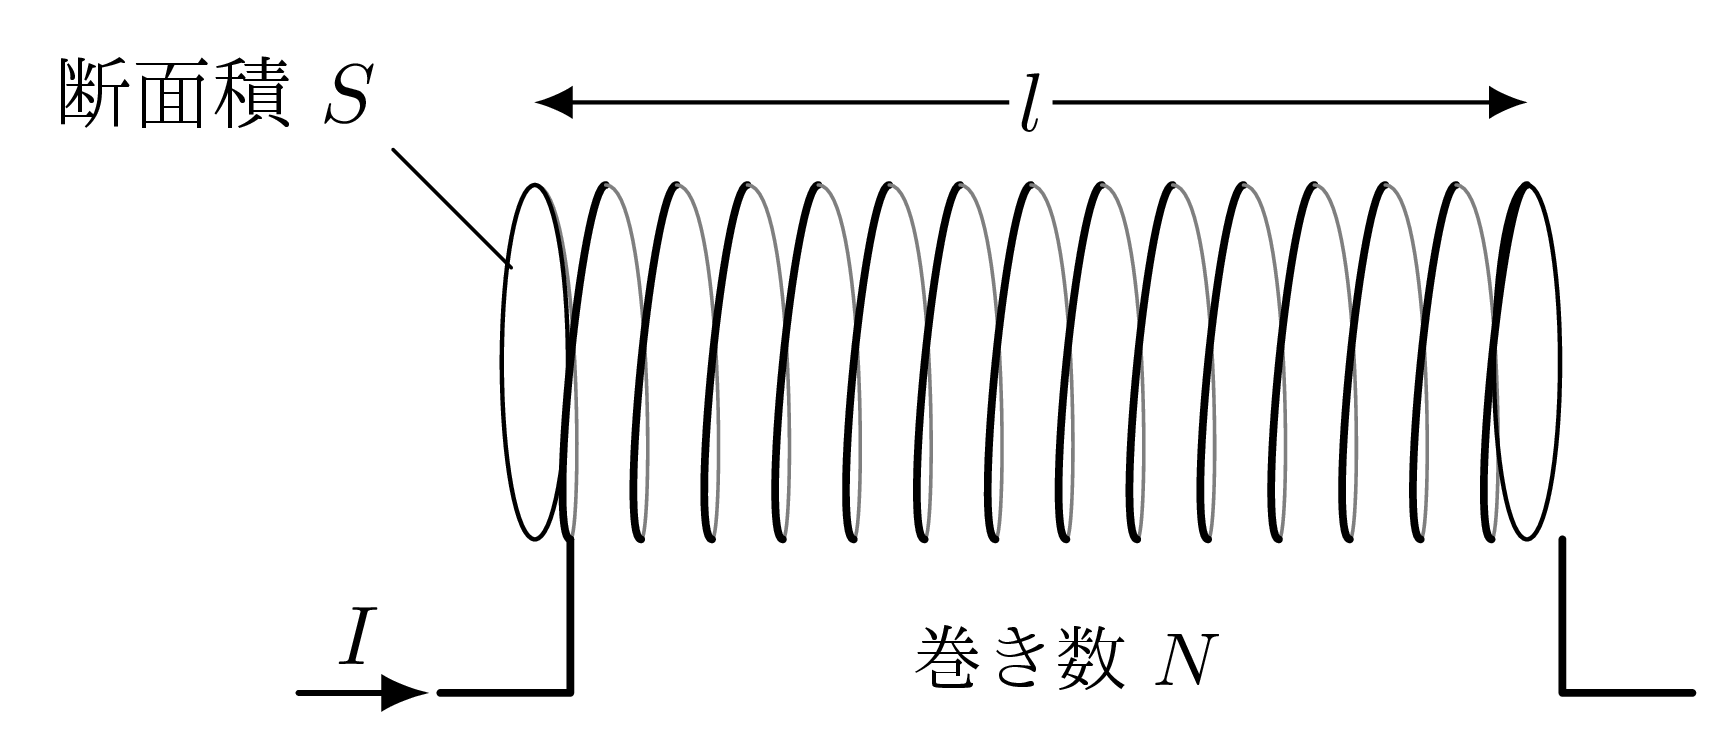
\includegraphics[keepaspectratio,width=60mm]{fig/n28_ex21_zu.png}
\end{zuright}
\end{reidai}

\begin{sisinE}
磁場$H$ → 磁束密度$B=\mu H$ → 磁束$\varPhi=BS$ の順に求める．
ソレノイドの磁場$H=n_0I$の$n_0$は{\gtfamily 単位長さあたりの巻き数}であり，全巻き数$N$ではない．
\end{sisinE}

\Key{$H=n_0I$\quad $B=\mu H$\quad $\varPhi=BS\cos\theta$}

\begin{kaitou}
単位長さあたりの巻き数は$n_0=\dfrac{N}{l}$なので，内部の磁場は$H=\dfrac{N}{l}I$．内部の磁束密度は一様で軸に平行なので，断面を貫く磁束は
\Ana{\varPhi=BS=\mu HS=\frac{\mu NIS}{l}\U{Wb}\Ans}
\end{kaitou}
\end{reidaiunit}

\subsection{電流が作る磁場}

磁場は磁極によって作られるほかに，{\gtfamily 電流が流れることによっても発生する}．
導線の形によって磁場の形・強さは変わり，一般にはビオ・サバールの法則$dH=\dfrac{1}{4\pi}\dfrac{I\sin\theta}{r^2}dx$で求められるが，これを実際に計算するのは容易ではない．
高校範囲では，次の3つの場合の磁場の形と強さを覚えておけばよい．向きはいずれも{\gtfamily 右ねじの法則}（電流の向きに右ねじを進めるとき，ねじを回す向きに磁場ができる）で決まる．

\begin{zuright}{52mm}
\noindent\MARU{1}\ {\gtfamily 直線電流の作る磁場}

\hspace{1zw}無限に長い直線導線に電流$I\U{A}$が流れているとき，導線を中心とする同心円状の磁場が発生し，磁場は円の接線方向を向く．中心から距離$r\U{m}$の位置での大きさは
\[H=\frac{I}{2\pi r}\U{A/m}\]
で，向きは{\gtfamily 右ねじを回す向き}である．
\zusep

\includegraphics[keepaspectratio,width=50mm]{text2_p62_fig1.png}
\end{zuright}

\begin{zuright}{52mm}
\noindent\MARU{2}\ {\gtfamily 円形電流の作る磁場}

\hspace{1zw}半径$r\U{m}$の円形の導線に電流$I\U{A}$が流れているとき，{\gtfamily 円の中心}における磁場の強さは
\[H=\frac{I}{2r}\U{A/m}\]
であり，向きは円の面に垂直で右ねじの法則で決まる（これ以外の点の磁場は簡単には求められない）．
円形の導線が$N$回巻いてあれば$H=N\dfrac{I}{2r}$となる．
\zusep

\includegraphics[keepaspectratio,width=50mm]{text2_p62_fig2.png}
\end{zuright}

\begin{zuright}{52mm}
\noindent\MARU{3}\ {\gtfamily ソレノイドの作る磁場}

\hspace{1zw}密に巻いた十分に長いコイルを{\gtfamily ソレノイド}という．ソレノイドに電流$I\U{A}$が流れているとき，{\gtfamily 内部全体に中心軸に平行な一様な磁場}が発生する．
単位長さ$1\U{m}$あたりの巻き数を$n_0\U{/m}$とすると，その強さは
\[H=n_0I\U{A/m}\]
であり，向きは右ねじの法則で決まる．ソレノイドの{\gtfamily 外部には磁場は発生しない}．
\zusep

\includegraphics[keepaspectratio,width=50mm]{text2_p62_fig3.png}
\end{zuright}

どの式からも分かるように，$\U{A}$を$\U{m}$で割った$\U{A/m}$が磁場の単位になっている．

\bsNeed{34mm}
\begin{matome}{電流の作る磁場}
 \hspace{3mm} 直線電流：$H=\dfrac{I}{2\pi r}$\hspace{8mm}
 円形電流（中心）：$H=\dfrac{I}{2r}$\hspace{8mm}
 ソレノイド（内部）：$H=n_0I$\\[1mm]
 \hspace{3mm} 向きはいずれも\AnaB{右ねじの法則}で決める．単位は$\U{A/m}$
\end{matome}

% 加筆：重ね合わせと，平面内の電流が作る磁場の向き・円弧の磁場（練習［82］［83］［88］）．
複数の電流があるときは，それぞれの電流が作る磁場を{\gtfamily ベクトルとして足し合わせる}（重ね合わせの原理）．
直線電流の磁場は，導線とその点を結ぶ線分に垂直な向きになることに注意して，向きを図に描いてから合成するとよい．

また，ある平面内を流れる電流がその平面内の点に作る磁場は，導線の形によらず{\gtfamily その平面に垂直}になる（導線を細かく区切り，各部分が作る磁場を考えれば分かる）．
例えば，中心角$\alpha$の円弧（半径$r$）を流れる電流が中心に作る磁場は，円全体の$\dfrac{\alpha}{2\pi}$倍，すなわち$\dfrac{\alpha}{2\pi}\cdot\dfrac{I}{2r}$である．
円周を等分した各部分は中心に対して同じ条件にあるので，同じ大きさの磁場を作るからである（練習［88］）．

%%%%%%%%%%  例題22（原本の【例題25】）  %%%%%%%%%%%%%%%%%%%%
\bsNeed{70mm}
\begin{reidaiunit}
\begin{reidai}{直線電流・円形電流の作る磁場}
\begin{zuright}{50mm}
\hspace{1zw}図のように，$xy$平面上に中心$\mathrm{O}$，半径$a\U{m}$の円形の導線があり，それが作る平面に垂直な（$z$軸に平行な）直線の導線が円に絶縁されて接している．それぞれに電流$I_1\U{A}$，$I_2\U{A}$が図の矢印の向きに流れている．図のように$x$，$y$，$z$軸の向きを取るものとして，以下の設問に答えよ．
\begin{komon}
\ko{1} 円形電流が中心$\mathrm{O}$に作る磁場の向きとその大きさを答えよ．
\ko{2} 直線電流が円形の中心$\mathrm{O}$に作る磁場の向きとその大きさを答えよ．
\ko{3} 点$\mathrm{O}$にできる合成磁場の大きさ，および合成磁場が$xy$平面となす角$\theta$の正接$\tan\theta$を求めよ．
\end{komon}
\zusep
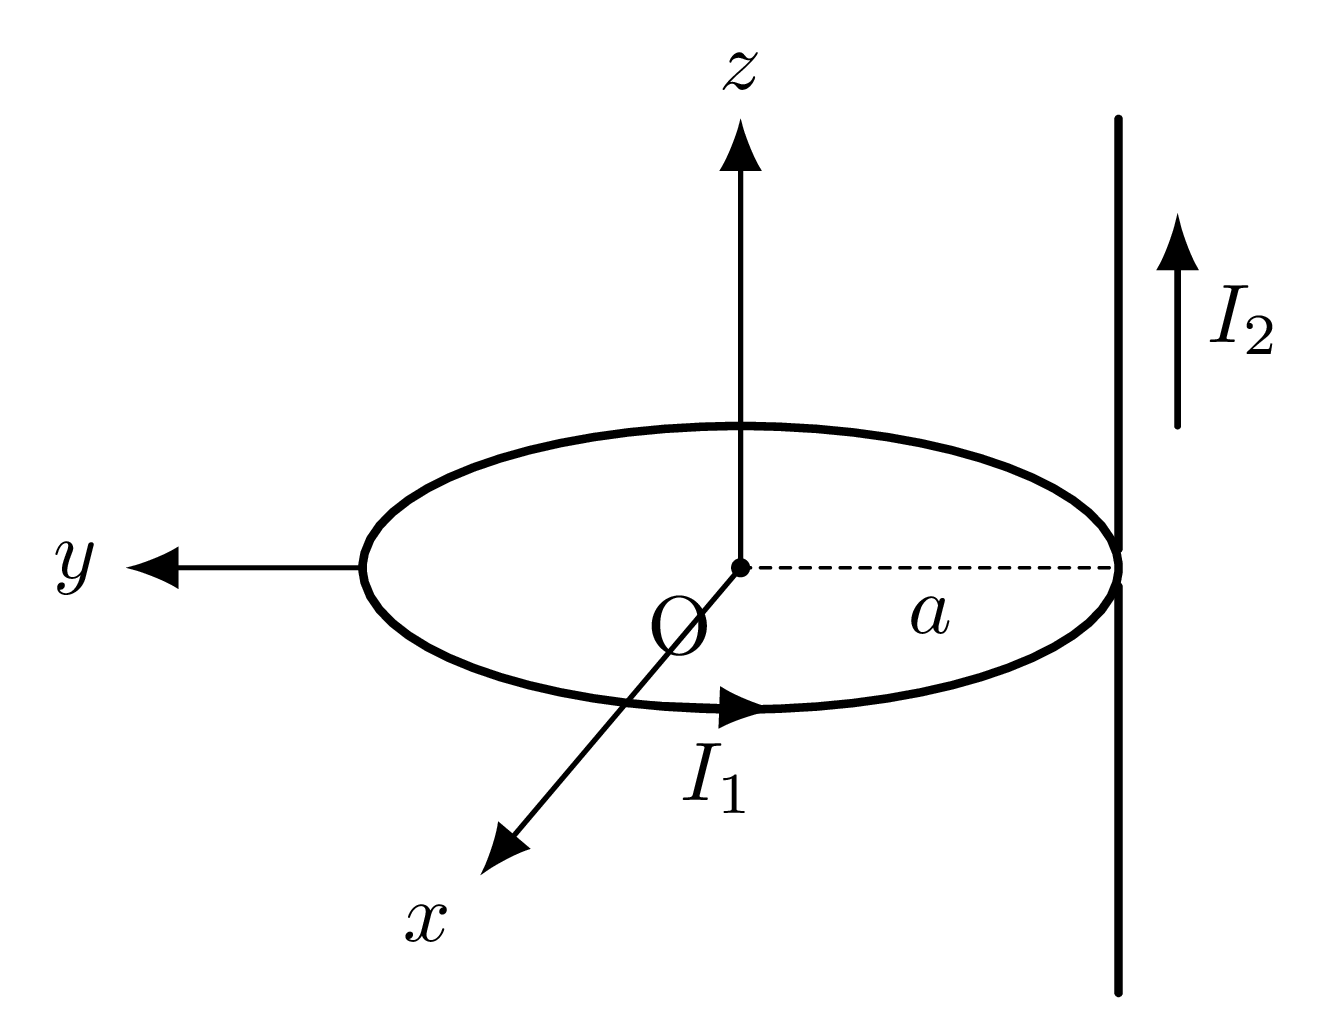
\includegraphics[keepaspectratio,width=48mm]{fig/n28_ex22_zu.png}
\end{zuright}
\end{reidai}

\begin{sisinE}
向きは右ねじの法則で決める．円形電流の中心の磁場は円の面に垂直（$z$軸方向），直線電流の磁場は直線に垂直な面内（$xy$平面内）にあり，互いに直交している．
2つの磁場は直交しているので，合成磁場の大きさは三平方の定理で求まる．
\end{sisinE}

\Key{直線電流の作る磁場$H=\dfrac{I}{2\pi r}$\quad 円形電流の作る磁場（中心）$H=\dfrac{I}{2r}$\quad 磁場はベクトルとして合成する}

\begin{kaitou}
\begin{komon}
\ko{1} 図の手前側（$+x$側）で電流は$-y$の向き（図の右向き）に流れているので，$+z$側から見て時計回りの電流である．右ねじの法則より磁場は$-z$の向きで，大きさは
       \[H_1=\frac{I_1}{2a}\U{A/m}\qquad(-z\ \text{の向き})\Ans\]
\ko{2} 直線導線は$\mathrm{O}$から$-y$の向きに距離$a$の位置にあり，電流は$+z$の向き．右ねじの法則より，$\mathrm{O}$での磁場は$-x$の向きで，大きさは
       \[H_2=\frac{I_2}{2\pi a}\U{A/m}\qquad(-x\ \text{の向き})\Ans\]
\ko{3} 2つの磁場は直交しているので
       \Ana{H=\sqrt{H_1^2+H_2^2}=\frac{\sqrt{\pi^2I_1^2+I_2^2}}{2\pi a}\U{A/m}\Ans}
       $xy$平面内の成分が$H_2$，垂直な成分が$H_1$なので
       \[\tan\theta=\frac{H_1}{H_2}=\frac{\pi I_1}{I_2}\Ans\]
       \begin{center}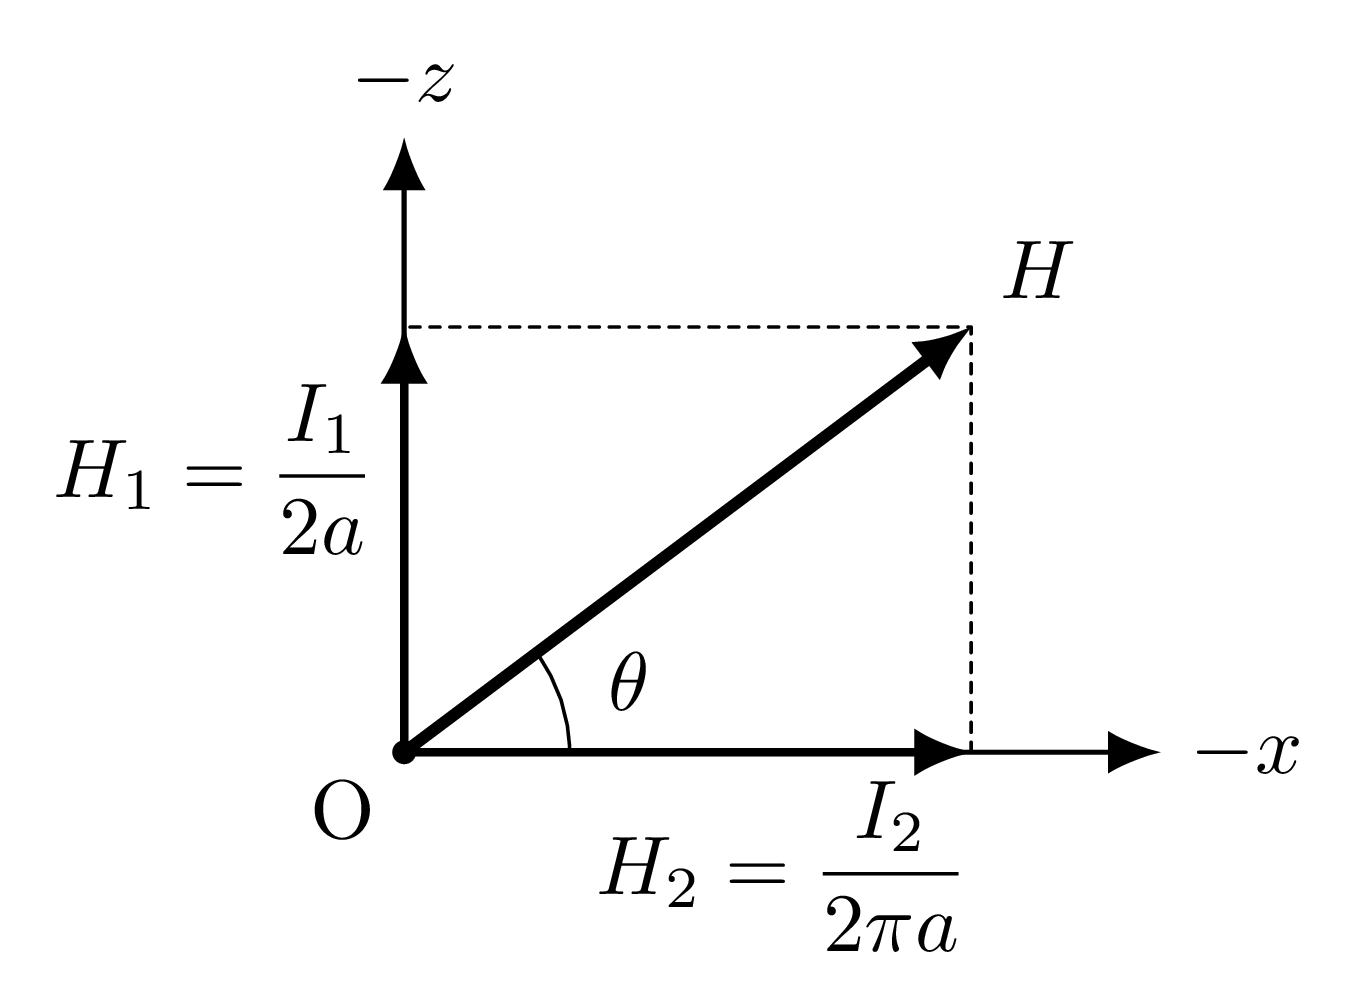
\includegraphics[keepaspectratio,width=44mm]{fig/n28_ex22_ans.png}\end{center}
\end{komon}
\end{kaitou}
\end{reidaiunit}

%%%%%%%%%%  例題23（原本の【例題26】）  %%%%%%%%%%%%%%%%%%%%
\bsNeed{66mm}
\begin{reidaiunit}
\begin{reidai}{平行導線の作る磁場の合成}
\begin{zuright}{54mm}
\hspace{1zw}$2a\U{m}$の間隔で平行に置かれた2本の無限に長い直線状の導線$\mathrm{A}$，$\mathrm{B}$に，それぞれ$I_{\mathrm{A}}$，$I_{\mathrm{B}}\U{A}$の電流が互いに逆向きに（$\mathrm{A}$は紙面の手前向き，$\mathrm{B}$は紙面の奥向きに）流れている．図のように$x$，$y$軸を設定するものとして，以下の設問に答えよ．
\begin{komon}
\ko{1} $I_{\mathrm{A}}>I_{\mathrm{B}}$であるとする．このとき，$x$軸上で合成磁場が$0\U{A/m}$となる点を求めよ．
\ko{2} $I_{\mathrm{A}}=I_{\mathrm{B}}=I\U{A}$のとき，図の点$\mathrm{P}(0,b)$に作られる磁場の大きさおよびその向きを求めよ．
\end{komon}
\zusep
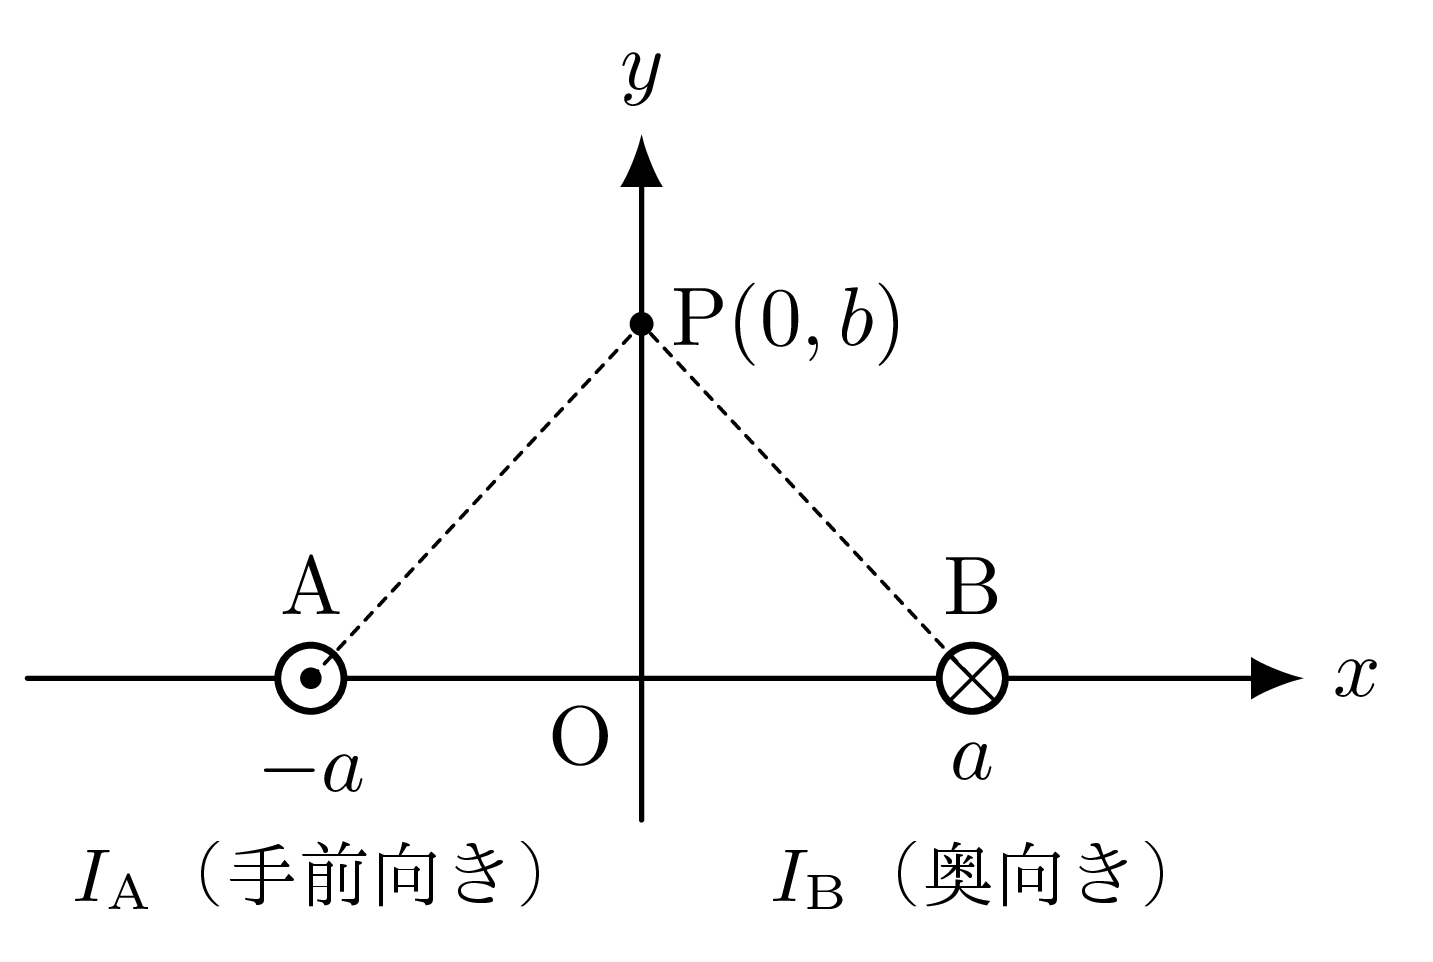
\includegraphics[keepaspectratio,width=52mm]{fig/n28_ex23_zu.png}
\end{zuright}
\end{reidai}

\begin{sisinE}
(1) 2つの磁場が打ち消し合うには，{\gtfamily 向きが逆で大きさが等しい}必要がある．逆向きの電流では，$\mathrm{A}$，$\mathrm{B}$の間では2つの磁場が同じ向きになるので，打ち消し合う点は外側にある．電流の小さい$\mathrm{B}$に近い側を調べる．

(2) 各電流が$\mathrm{P}$に作る磁場は，導線と$\mathrm{P}$を結ぶ線分に垂直である．向きを図に描き，成分に分けて足す．
\end{sisinE}

\Key{直線電流の磁場は導線と点を結ぶ線分に垂直\quad 磁場はベクトルとして合成する}

\begin{kaitou}
\begin{komon}
\ko{1} $\mathrm{A}$（手前向き）の磁場は$+z$から見て反時計回り，$\mathrm{B}$（奥向き）の磁場は時計回りである．$x$軸上の$-a<x<a$では両者とも$-y$の向きで打ち消さない．$x>a$では$\mathrm{A}$の磁場は$+y$，$\mathrm{B}$の磁場は$-y$の向きなので，大きさが等しくなる点で$0$になる：
       \Ana{\frac{I_{\mathrm{A}}}{2\pi(x+a)}=\frac{I_{\mathrm{B}}}{2\pi(x-a)}\qquad\therefore\ x=\frac{I_{\mathrm{A}}+I_{\mathrm{B}}}{I_{\mathrm{A}}-I_{\mathrm{B}}}a}
       （$x<-a$では$\mathrm{A}$に近く$I_{\mathrm{A}}>I_{\mathrm{B}}$なので打ち消さない．）よって
       \[\Bigl(\frac{I_{\mathrm{A}}+I_{\mathrm{B}}}{I_{\mathrm{A}}-I_{\mathrm{B}}}a,\ 0\Bigr)\Ans\]
\ko{2} $\mathrm{AP}=\mathrm{BP}=\sqrt{a^2+b^2}$なので，各電流が$\mathrm{P}$に作る磁場の大きさはどちらも$H_0=\dfrac{I}{2\pi\sqrt{a^2+b^2}}$である．
       $\mathrm{A}$の磁場は$\overrightarrow{\mathrm{AP}}=(a,b)$に垂直で反時計回りの向き$(-b,a)$方向，$\mathrm{B}$の磁場は$\overrightarrow{\mathrm{BP}}=(-a,b)$に垂直で時計回りの向き$(b,a)$方向である．$x$成分は打ち消し，$y$成分は足し合わされるので
       \[H=2H_0\cdot\frac{a}{\sqrt{a^2+b^2}}=\frac{aI}{\pi(a^2+b^2)}\U{A/m}\qquad(+y\ \text{の向き})\Ans\]
\end{komon}
\end{kaitou}
\end{reidaiunit}

\subsection{電磁力}

\begin{zuright}{54mm}
\hspace{1zw}電流の流れている導線は，周りの磁場から力を受ける．この力を{\gtfamily 電磁力}という．
磁束密度$B\U{T}$の磁場中を，磁場と角$\theta$をなす方向に電流$I\U{A}$が流れるとき，導線の長さ$l\U{m}$の部分が受ける力の大きさは
\AnaBD{F=IBl\sin\theta\U{N}}
で与えられる（$B=\mu H$なので$F=\mu IHl\sin\theta$とも書ける）．
\zusep

\includegraphics[keepaspectratio,width=52mm]{text2_p64_fig1.png}
\end{zuright}

\begin{zuright}{46mm}
\hspace{1zw}$B\sin\theta$は，磁束密度の{\gtfamily 電流に垂直な成分}$B_\perp$である．すなわち，導線は磁場のうち電流と垂直な成分からだけ力を受け，
\[F=IB_\perp l\U{N}\]
となる．電流と平行な磁場からは力を受けない．

\hspace{1zw}電磁力の向きは{\gtfamily フレミングの左手の法則}で決める．左手の{\gtfamily 中指を電流の向き，人差し指を磁場の向き}に取ったとき，{\gtfamily 親指の向きが電磁力の向き}である．電磁力は電流にも磁場にも垂直である．
\zusep

\includegraphics[keepaspectratio,width=44mm]{text2_p64_fig2.png}\\[2mm]

\includegraphics[keepaspectratio,width=36mm]{text2_p64_fig3.png}
\end{zuright}

% 加筆：力の作用図（組版チェックリスト §2．練習［86］）．
電磁力を受けて静止している導体棒などでは，重力・垂直抗力・電磁力のつり合いを考える．
電磁力は電流と磁場の両方に垂直なので向きを取り違えやすい．{\gtfamily 電流の向きに沿って横から見た図を描き，はたらく力をすべて矢印で描き込んでから}つり合いの式を立てること（練習［86］の解答の図）．

\bsNeed{26mm}
\begin{matome}{電磁力}
 \hspace{3mm} 電流が磁場から受ける力\quad $F=IBl\sin\theta=IB_\perp l\U{N}$\\
 \hspace{3mm} 向きは\AnaB{フレミングの左手の法則}（中指：電流，人差し指：磁場，親指：力）
\end{matome}

%%%%%%%%%%  例題24（原本の【例題27】）  %%%%%%%%%%%%%%%%%%%%
\bsNeed{60mm}
\begin{reidaiunit}
\begin{reidai}{平行導線の及ぼし合う電磁力}
\begin{zuright}{40mm}
\hspace{1zw}図のように，真空中に距離$r\U{m}$だけ離れた2本の無限に長い直線状の導線$\mathrm{A}$，$\mathrm{B}$があり，それぞれに大きさ$I_1\U{A}$，$I_2\U{A}$の電流が同じ向き（紙面の奥から手前の向き）に流れている．真空の透磁率を$\mu_0\U{Wb^2/N\cdot m^2}$として以下の設問に答えよ．なお，図中の記号$\odot$は電流が紙面の手前側に向かって流れていることを，記号$\otimes$は紙面奥側に向かって流れていることを意味する．
\zusep
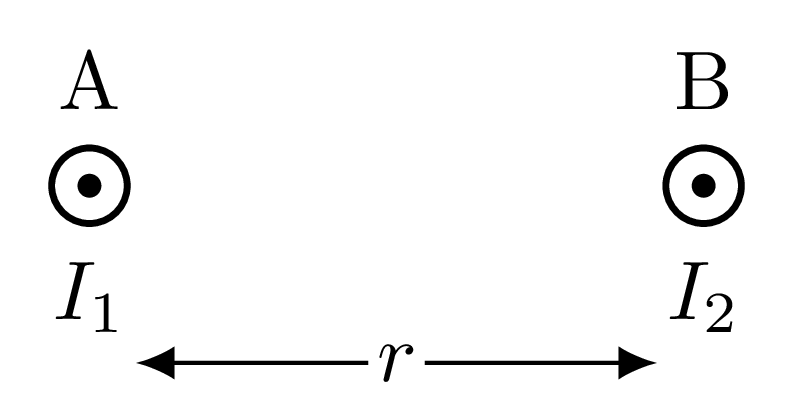
\includegraphics[keepaspectratio,width=36mm]{fig/n28_ex24_zu.png}
\end{zuright}
\begin{komon}
\ko{1} $\mathrm{A}$の電流が，導線$\mathrm{B}$の位置に作る磁束密度の向きおよび大きさを求めよ．
\ko{2} 導線$\mathrm{B}$の長さ$l\U{m}$の部分が$\mathrm{A}$の電流から受ける力の向きおよび大きさを求めよ．
\ko{3} $\mathrm{B}$の電流が，導線$\mathrm{A}$の位置に作る磁束密度の向きおよび大きさを求めよ．
\ko{4} 導線$\mathrm{A}$の長さ$l\U{m}$の部分が導線$\mathrm{B}$の電流から受ける力の向きおよび大きさを求めよ．
\ko{5} $\mathrm{B}$を流れる電流が逆向き（紙面の手前から奥の向き）であるとき，$\mathrm{B}$の長さ$l\U{m}$の部分が導線$\mathrm{A}$の電流から受ける力の向きおよび大きさを求めよ．
\end{komon}
\end{reidai}

\begin{sisinE}
一方の電流が作る磁場の中に，もう一方の電流が置かれていると考える．
磁場は右ねじの法則で，力の向きはフレミングの左手の法則で決める．
(2)と(4)は作用・反作用の関係にある．
\end{sisinE}

\Key{直線電流の作る磁場$H=\dfrac{I}{2\pi r}$\quad 電磁力$F=IBl\sin\theta$\quad 力の向きはフレミングの左手の法則}

\begin{kaitou}
\begin{komon}
\ko{1} $\mathrm{A}$の電流（手前向き）は反時計回りの磁場を作るので，$\mathrm{B}$の位置では{\gtfamily 図の上向き}で，大きさは
       \[B_1=\mu_0\frac{I_1}{2\pi r}\U{T}\Ans\]
\ko{2} $\mathrm{B}$の電流（手前向き）と上向きの磁場にフレミングの左手の法則を用いると，力は{\gtfamily $\mathrm{A}$に向かう向き（左向き）}である．電流と磁場は垂直なので
       \Ana{F=I_2B_1l=\frac{\mu_0I_1I_2l}{2\pi r}\U{N}\Ans}
       \begin{center}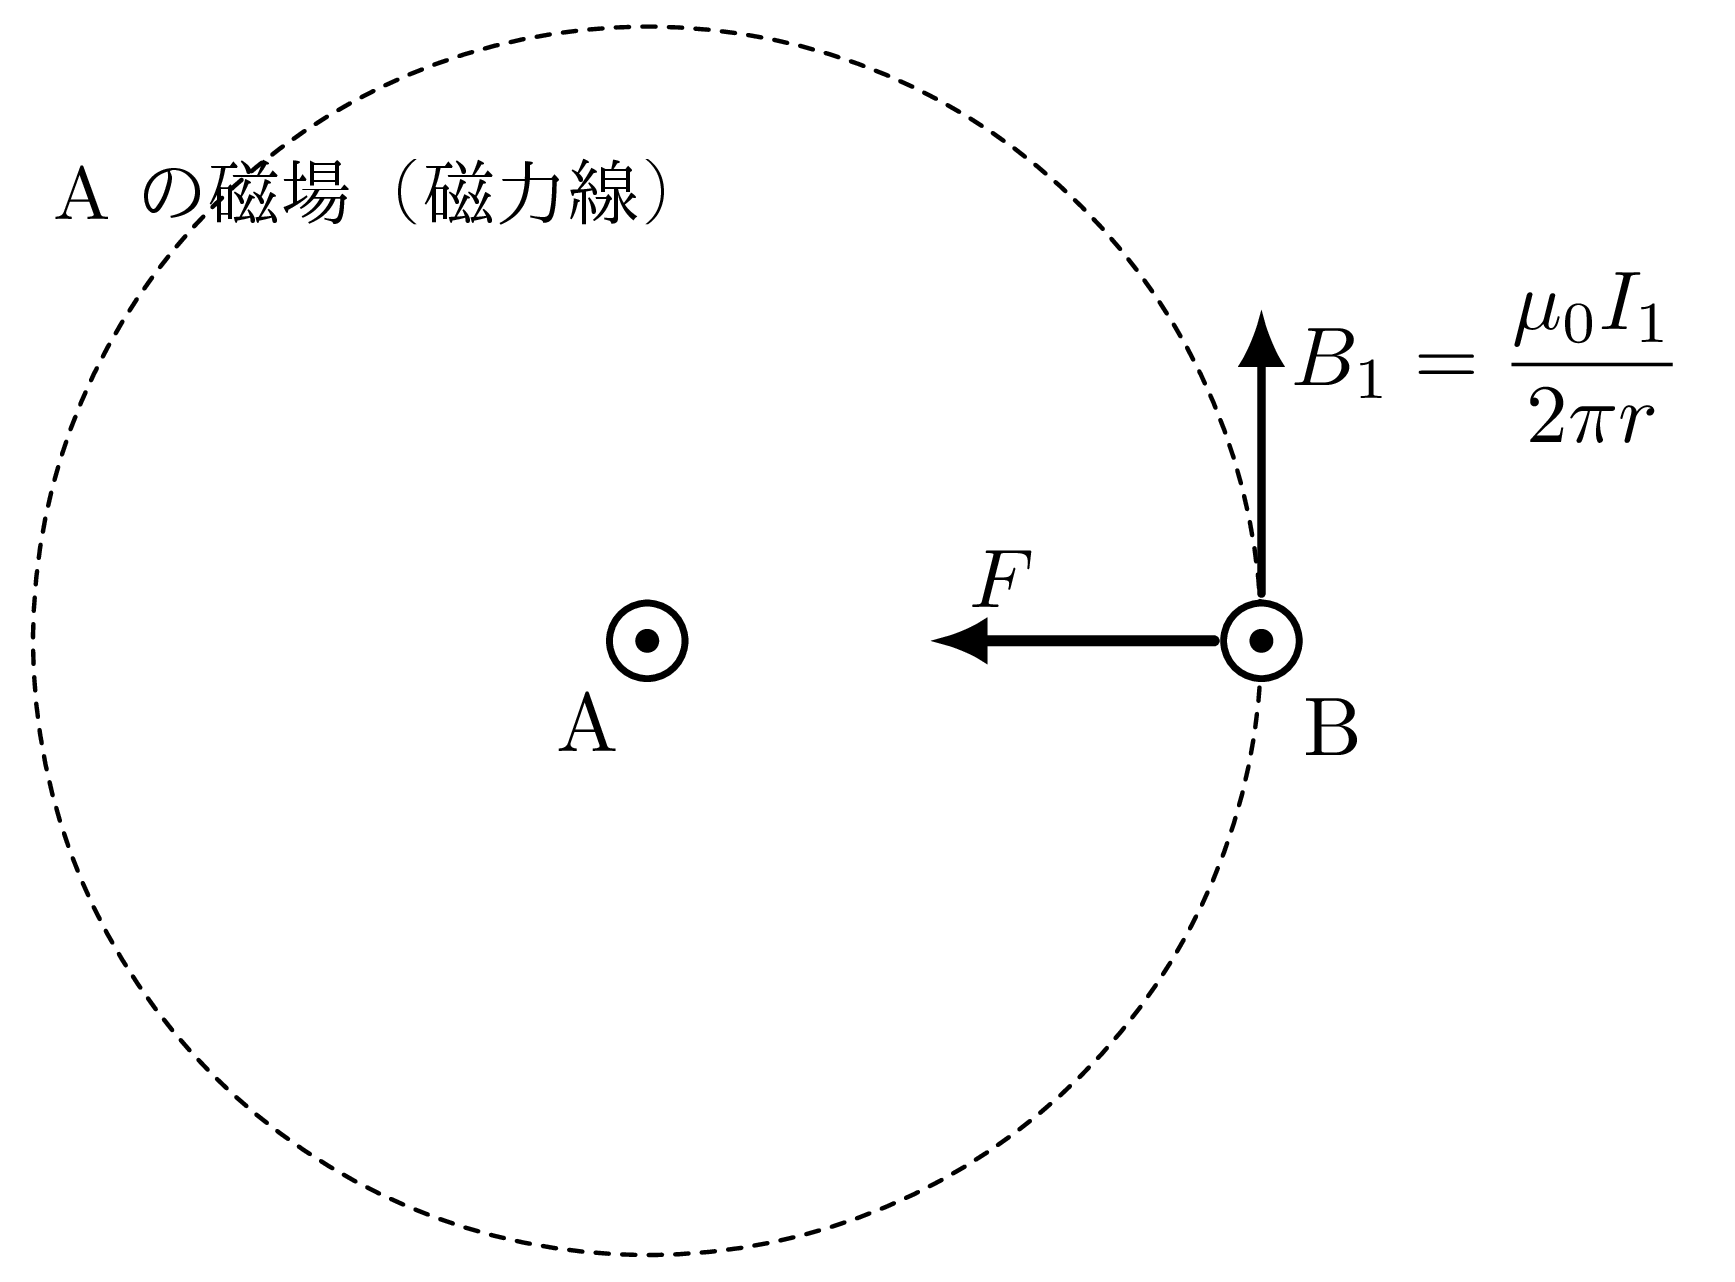
\includegraphics[keepaspectratio,width=44mm]{fig/n28_ex24_ans.png}\end{center}
\ko{3} 同様に，$\mathrm{A}$の位置では{\gtfamily 図の下向き}で
       \[B_2=\mu_0\frac{I_2}{2\pi r}\U{T}\Ans\]
\ko{4} 力は{\gtfamily $\mathrm{B}$に向かう向き（右向き）}で，
       \[F=I_1B_2l=\frac{\mu_0I_1I_2l}{2\pi r}\U{N}\Ans\]
       （(2)と大きさが等しく向きが逆で，作用・反作用の法則を満たしている．）
\ko{5} $\mathrm{B}$の電流の向きが逆になるので，力の向きも逆になり，{\gtfamily $\mathrm{A}$から遠ざかる向き（右向き）}に大きさ
       \[F=\frac{\mu_0I_1I_2l}{2\pi r}\U{N}\Ans\]
\end{komon}
\end{kaitou}
\end{reidaiunit}

例題24 より，次のことが分かる．

\bsNeed{30mm}
\begin{matome}{平行電流にはたらく力}
 \hspace{3mm} 距離$r$だけ離れた平行電流$I_1$，$I_2$の長さ$l$の部分にはたらく力の大きさは
 \AnaBD{F=\frac{\mu_0I_1I_2}{2\pi r}l\U{N}}
 \hspace{3mm} {\gtfamily 同じ向きの電流は引き合い，逆向きの電流は反発し合う}
\end{matome}

\newpage

%%%%%%%%%%%%%%%%%%%%  練習問題  %%%%%%%%%%%%%%%%%%%%
% 第27回の［80］に続く．
\setcounter{qno}{80}

\filbreak
\Rank{A問題}

\Mon{基本公式の確認}

\hspace{1zw}以下の設問に答えよ．ただし真空の透磁率を$\mu_0=4\pi\times 10^{-7}\U{Wb/A\cdot m}$とする．
\begin{komon}
\ko{1} 強さ$100\U{N/Wb}$の磁場中に磁極を置いたところ，大きさ$0.5\U{N}$の力を受けた．この磁極の強さは何$\U{Wb}$か．
\ko{2} 真空中で，強さ$10\U{N/Wb}$の磁場に対して垂直な面積$100\U{cm^2}$の断面を貫く磁束は何$\U{Wb}$か．
\ko{3} 長さ$20\U{cm}$，総巻数$500$回の密に巻いたソレノイド・コイルに，強さ$4.0\U{A}$の電流を流したときコイル内部に生じる磁場の強さは何$\U{A/m}$か．
\ko{4} 無限に長い直線導線に強さ$3.0\U{A}$の電流が流れているとき，この導線から$50\U{cm}$だけ離れたところにおける磁場の強さは何$\U{A/m}$か．
\ko{5} 半径$10\U{cm}$の円形導線に強さ$4.0\U{A}$の電流が流れているとき，この円の中心における磁場の強さは何$\U{A/m}$か．
\end{komon}

\filbreak
\Rank{B問題}

\Mon[\Sitei]{直線電流・円形電流の作る磁場}

\begin{zuright}{62mm}
\hspace{1zw}次の\framebox[4zw]{\rule{0pt}{1.1zw}1}から\framebox[4zw]{\rule{0pt}{1.1zw}5}に当てはまる適当な語句および数値を入れよ．
\par
\hspace{1zw}右図のように紙面上に平行な長い直線導線$\mathrm{A}$，$\mathrm{B}$と半径$a\U{m}$のひと巻きの円形コイルが固定されている．$\mathrm{A}$，$\mathrm{B}$間の距離は$2d\U{m}$で，円形コイルの中心点$\mathrm{O}$は2本の平行直線導線のちょうど中間の位置にある．
\zusep
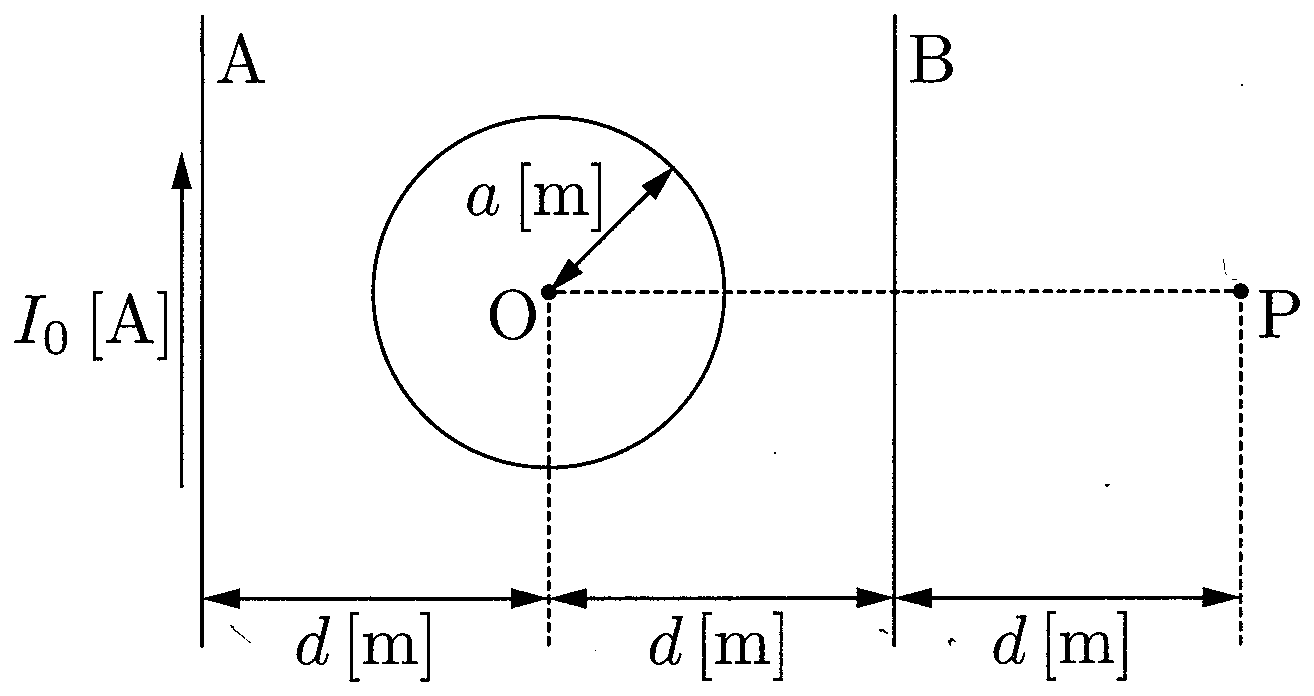
\includegraphics[keepaspectratio,width=60mm]{fig/n28_p82_zu.png}
\end{zuright}
\hspace{1zw}今，円形コイルには電流を流さず，直線導線$\mathrm{A}$のみに矢印の向きに強さ$I_0\U{A}$の電流を流す．次に直線導線$\mathrm{B}$に強さ\framebox[4zw]{\rule{0pt}{1.1zw}1}$\U{A}$の電流を\framebox[4zw]{\rule{0pt}{1.1zw}2}向きに流すと，$\mathrm{B}$の右側の距離$d\U{m}$にある点$\mathrm{P}$の磁場は$0\U{A/m}$となる．このとき，コイルの中心点$\mathrm{O}$の磁場の向きは\framebox[4zw]{\rule{0pt}{1.1zw}3}である．この状態において，点$\mathrm{O}$の合成磁場を$0\U{A/m}$にするには，円形コイルに強さ\framebox[4zw]{\rule{0pt}{1.1zw}4}$\U{A}$の電流を\framebox[4zw]{\rule{0pt}{1.1zw}5}向きに流せばよい．

\Mon{平行電流の作る磁場の合成}

\begin{zuright}{50mm}
\hspace{1zw}右図のように，紙面上に点$\mathrm{O}$を原点とする$x$-$y$座標系をとる．点$\mathrm{A}(-a,0)\U{m}$，$\mathrm{B}(a,0)\U{m}$には十分長い2本の細い導線が紙面に垂直に張られており，$\mathrm{A}$については紙面手前向きに，また$\mathrm{B}$については紙面向こう向きに，それぞれ強さ$I_1\U{A}$，$I_2\U{A}$の電流が流れている．これについて以下の設問に答えよ．
\begin{komon}
\ko{1} $\mathrm{A}$，$\mathrm{B}$点の間にある$x$軸上の点$\mathrm{P}(x,0)$（$-a<x<a$）における磁場の強さおよび向きを求めよ．
\ko{2} 点$\mathrm{Q}(a,a)$における磁場の向きを測定したところ，$y$軸に平行であった．このことから，二つの電流の強さの比$\dfrac{I_1}{I_2}$を求めよ．
\end{komon}
\zusep
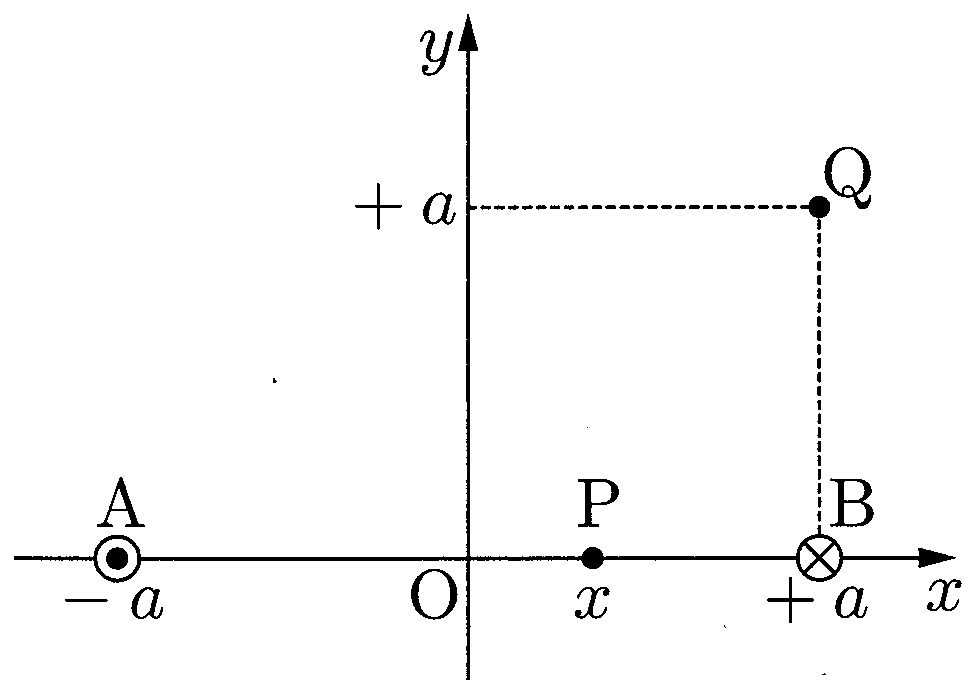
\includegraphics[keepaspectratio,width=48mm]{fig/n28_p83_zu.png}
\end{zuright}

\Mon{ソレノイドコイル}

\hspace{1zw}長さ$0.20\U{m}$，巻数$3000$回のコイルを南北に平行に，地面に対して水平に置く．地磁気の水平分力（水平方向の成分）が$24\U{A/m}$であるとき，コイルの中心位置での合成磁場を$0$とするためにはこのコイルにどれだけの電流を流せばよいか．

\Mon{直線電流の作る磁場}

\begin{zuright}{50mm}
\hspace{1zw}2本の無限に長い導線$\mathrm{A}$，$\mathrm{B}$を図に示すような位置関係に配置する（ただし図の$xy$平面が地面に対して平行な水平面である）．最初，導線$\mathrm{B}$に$y$軸負の向きに強さが$I_0\U{A}$一定の電流を流しておく．次に，導線$\mathrm{A}$に$x$軸負の向きの電流を流し，その強さをゆっくりと$0\U{A}$から$I_0\U{A}$まで増加させた．このとき，原点の位置に水平に置かれた磁針のN極と$x$軸の正の向きがなす角は何度から何度まで変化するかを求めよ．ただし，地磁気の影響は無視してよいものとする．
\zusep
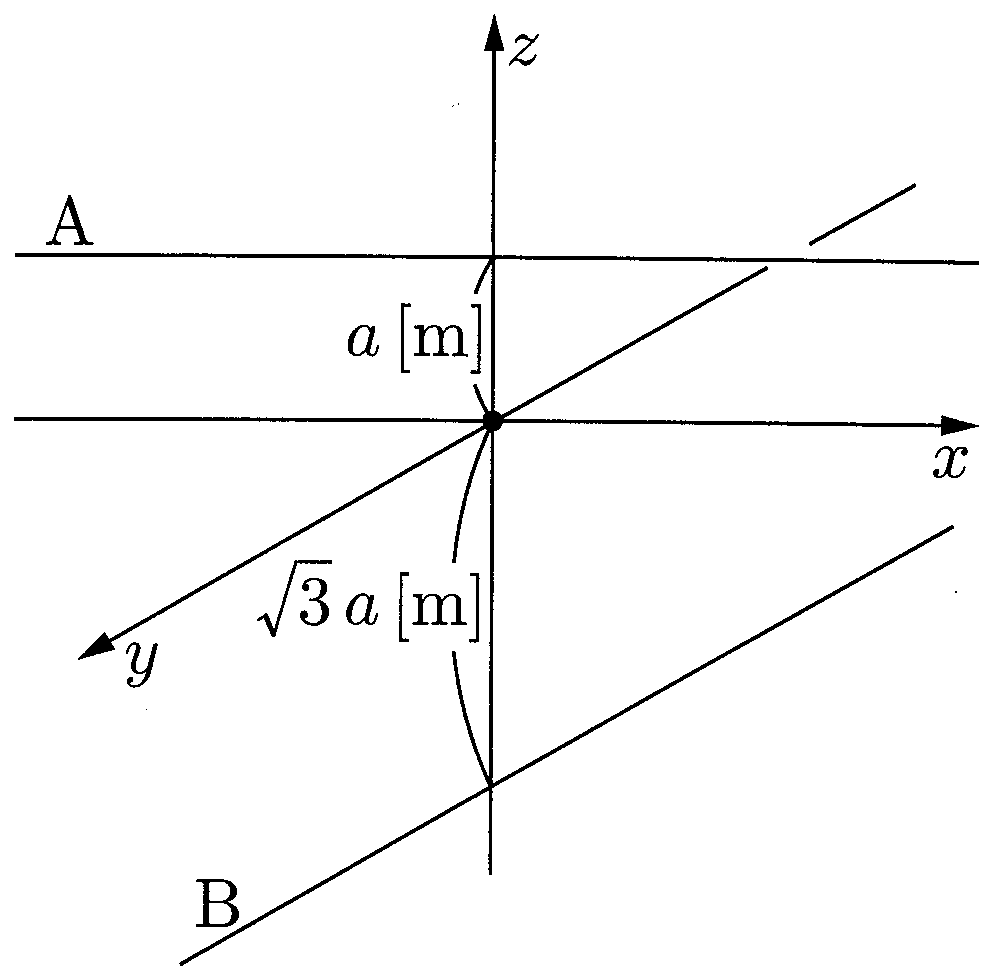
\includegraphics[keepaspectratio,width=48mm]{fig/n28_p85_zu.png}
\end{zuright}

\Mon[\Sitei]{電磁力}

\begin{zuright}{60mm}
\hspace{1zw}右図のように鉛直下向きに強さ$H\U{A/m}$の一様な磁場中で，水平と$\theta\U{rad}$の傾きをなして2本の導線$\mathrm{A}$，$\mathrm{B}$を間隔$d\U{m}$で平行に固定し，この上に質量$m\U{kg}$の導体棒$\mathrm{PQ}$をのせる．今$\mathrm{A}$，$\mathrm{B}$間に適当な向きに電池と抵抗をつないで$\mathrm{PQ}$に電流を流したところ，$\mathrm{PQ}$は2本の導線に対して垂直をなして図のように静止した．真空の透磁率を$\mu_0\U{N/A^2}$，重力加速度の大きさを$g\U{m/s^2}$として以下の問いに答えよ．
\begin{komon}
\ko{1} $\mathrm{PQ}$に流した電流の向きを求めよ．
\ko{2} $\mathrm{PQ}$に流した電流の強さ$I\U{A}$を求めよ．
\end{komon}
\zusep
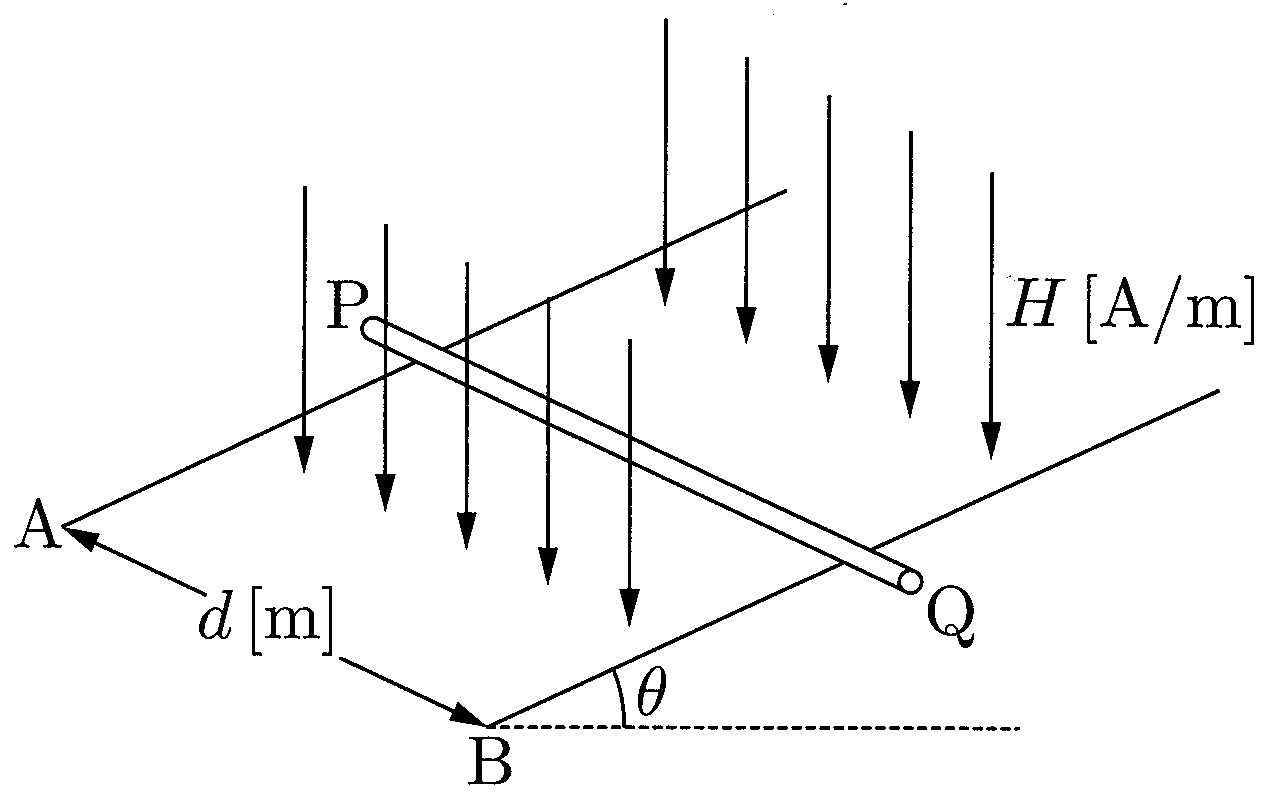
\includegraphics[keepaspectratio,width=58mm]{fig/n28_p86_zu.png}
\end{zuright}

\Mon{平行導線間の力}

\begin{zuright}{44mm}
\hspace{1zw}右図のような一辺$a\U{m}$の正方形$\mathrm{ABCD}$の各頂点に，紙面に対して垂直にそれぞれ強さ$I\U{A}$の電流が流れている．電流の向きは$\mathrm{A}$，$\mathrm{D}$にある導線には紙面の表→裏向き，また$\mathrm{B}$，$\mathrm{C}$にある導線には裏→表向きである．真空の透磁率を$\mu_0\U{N/A^2}$として以下の問いに答えよ．
\begin{komon}
\ko{1} 正方形の中心$\mathrm{O}$における磁場の強さ$H_{\mathrm{O}}\U{A/m}$を求めよ．
\ko{2} $\mathrm{C}$にある導線の単位長さ$1\U{m}$当たりに働く力の大きさ$f_{\mathrm{C}}\U{N}$を求めよ．
\end{komon}
\zusep
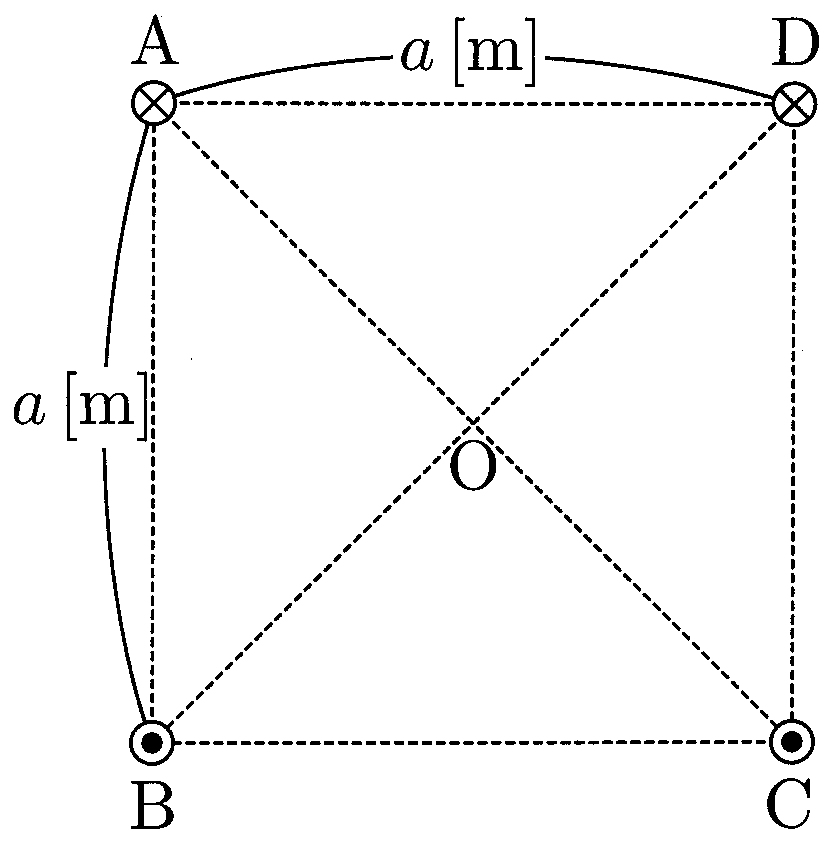
\includegraphics[keepaspectratio,width=40mm]{fig/n28_p87_zu.png}
\end{zuright}

\filbreak
\Rank{C問題}

\Mon{部分円電流の作る磁場}

\hspace{1zw}強さ$I\U{A}$の電流が流れている(1)(2)の回路について，点$\mathrm{O}$における磁場の大きさ$H\U{A/m}$をそれぞれ求めよ．ただし(2)については，半円の下の導線は無限遠方まで伸びている直線導線である．また点$\mathrm{O}$における磁場は導線が作る平面に対して垂直になっていることを証明なしに利用してよい．
\begin{center}
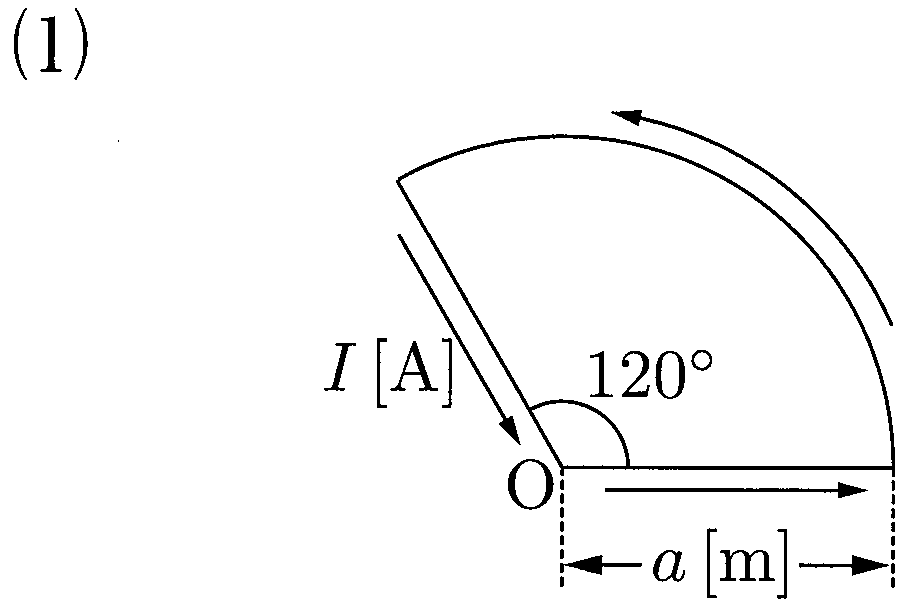
\includegraphics[keepaspectratio,width=46mm]{fig/n28_p88_zu1.png}\hspace{14mm}%
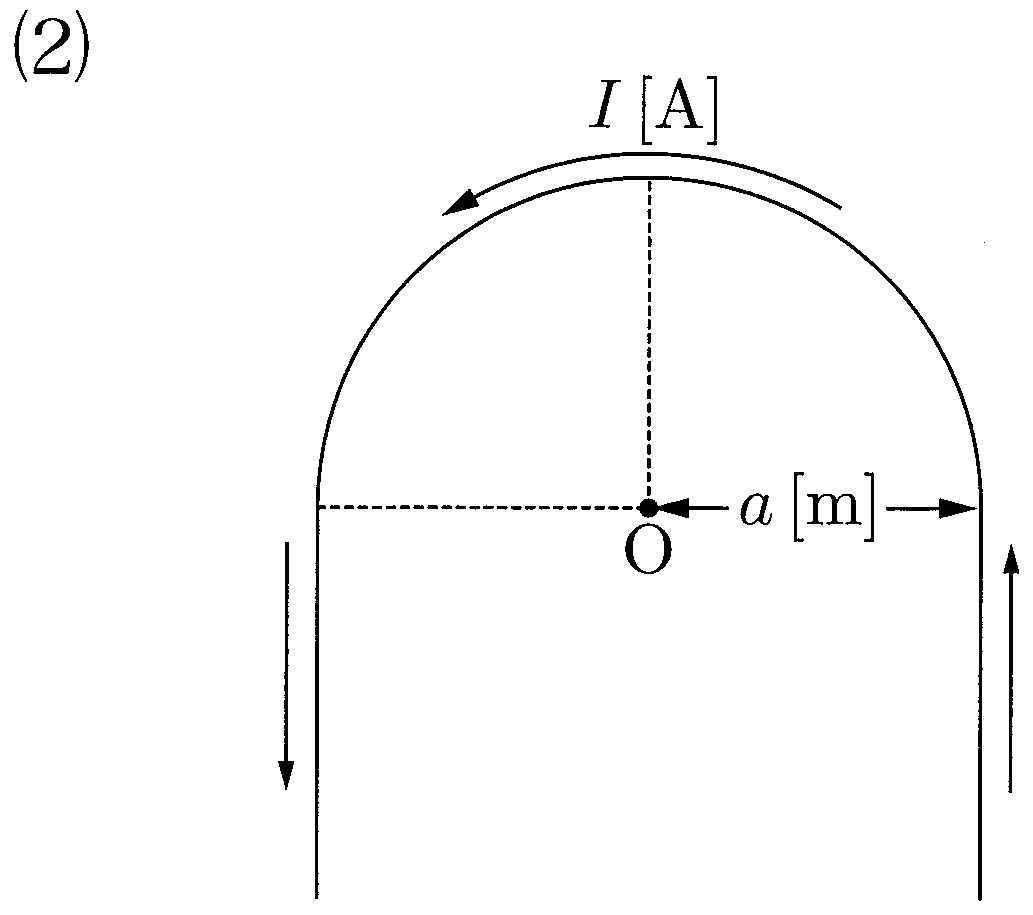
\includegraphics[keepaspectratio,width=50mm]{fig/n28_p88_zu2.png}
\end{center}

\Mon{長方形コイルが受ける力}

\begin{zuright}{60mm}
\hspace{1zw}右図のように十分長い導線$\mathrm{PQ}$と長方形のコイル$\mathrm{ABCD}$を同一平面内に固定し，導線，コイルにそれぞれ強さ$I_1$，$I_2\U{A}$の電流を右図の矢印の向きに流した．$\overline{\mathrm{AB}}=a\U{m}$，$\overline{\mathrm{BC}}=b\U{m}$であり，また$\mathrm{PQ}$と$\mathrm{AB}$とは平行でその間隔は$d\U{m}$である．真空の透磁率を$\mu_0\U{N/A^2}$として以下の問いに答えよ．
\begin{komon}
\ko{1} 導線$\mathrm{PQ}$が辺$\mathrm{AB}$，$\mathrm{CD}$に及ぼす力の大きさ$f_{\mathrm{AB}}$，$f_{\mathrm{CD}}\U{N}$をそれぞれ求めよ．
\ko{2} 導線$\mathrm{PQ}$が長方形コイル$\mathrm{ABCD}$に及ぼす合力の向きおよび大きさを求めよ．
\end{komon}
\zusep
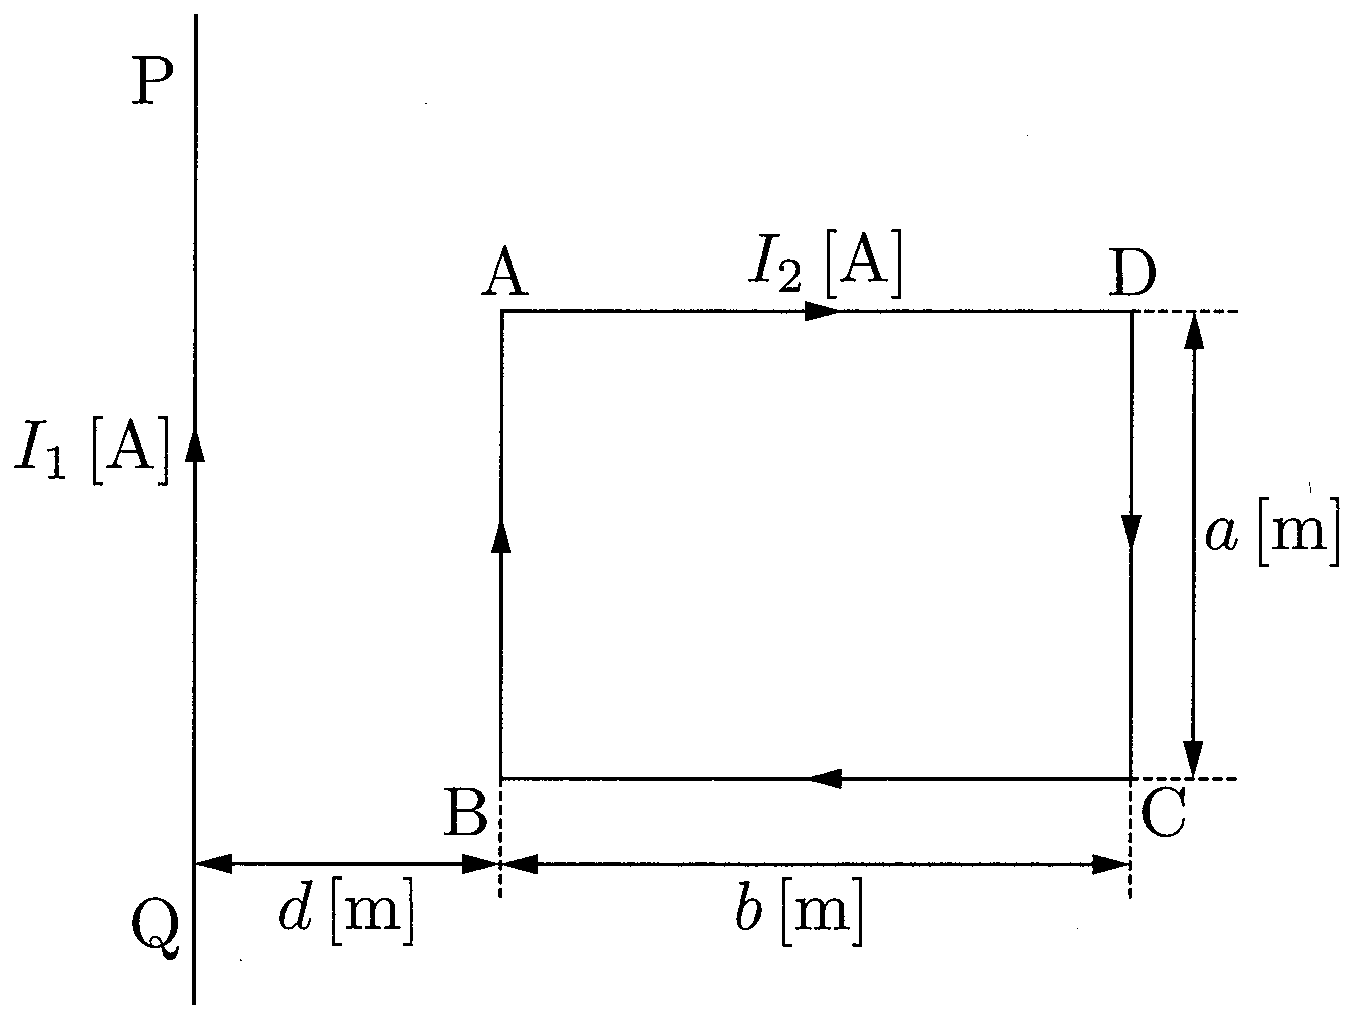
\includegraphics[keepaspectratio,width=58mm]{fig/n28_p89_zu.png}
\end{zuright}

\newpage

%%%%%%%%%%%%%%%%%%%%  解答  %%%%%%%%%%%%%%%%%%%%
\KaiTitle{第28回　電流のつくる磁場と電磁力}
\setlength{\columnseprule}{0.4pt}
\begin{multicols}{2}
\raggedcolumns

\Rank{A問題}
\MonN{81}{基本公式の確認}\par\nopagebreak
\begin{sisin}
直線電流，円形電流の作る磁場の式はよく似ているので間違えないように注意せよ．また，磁場，磁束密度，磁束の三つを取り違えないように注意すること．磁場は$H\U{A/m}$，磁束密度は$B\U{Wb/m^2}$，磁束は$\varPhi\U{Wb}$であり，$B=\mu_0H$，$\varPhi=BS\cos\theta$の関係式で結ばれている．単位まで含めてきちんと覚えておこう．

なお，磁場を表す単位は，$\U{N/Wb}$でも$\U{A/m}$でもよいが$\U{A/m}$を用いることが多い．
\end{sisin}
\KaiHead
\begin{komon}
\ko{1} $F=mH$であるから，
       \[m=\frac{0.5}{100}=5.0\times 10^{-3}\U{Wb}\Ans\]
\ko{2} \[\begin{aligned}
         \varPhi&=BS=(\mu_0H)\cdot S\\
          &=4\pi\times 10^{-7}\cdot 10\cdot 100\times 10^{-4}\\
          &\fallingdotseq 1.3\times 10^{-7}\U{Wb}\Ans
       \end{aligned}\]
\ko{3} \[\begin{aligned}H&=n_0I=\frac{500}{20\times 10^{-2}}\cdot 4.0\\&=1.0\times 10^4\U{A/m}\Ans\end{aligned}\]
\ko{4} \[\begin{aligned}H&=\frac{I}{2\pi r}=\frac{3.0}{2\pi\cdot 0.50}\\&\fallingdotseq 9.5\times 10^{-1}\U{A/m}\Ans\end{aligned}\]
\ko{5} \[H=\frac{I}{2r}=\frac{4.0}{2\cdot 0.10}=2.0\times 10\U{A/m}\Ans\]
\end{komon}

\Rank{B問題}
\MonN[\Sitei]{82}{直線電流・円形電流の作る磁場}\par\nopagebreak
\begin{sisin}
磁場を合成する際には，ベクトル合成をする，すなわち向きを考えた上で足し合わせを行う必要がある．右ねじの法則をきちんと考えながら合成を行おう．
\end{sisin}
\KaiHead
\begin{komon}
\item[{\makebox[1.9zw][r]{(1)(2)}}] 右ねじの法則より，直線導線$\mathrm{A}$に流れる電流が点$\mathrm{P}$に作る磁場の向きは紙面に対して表→裏の向きとなり，その磁場の強さは
       \[H_{\mathrm{AP}}=\frac{I_0}{2\pi(3d)}\U{A/m}\]
       である．よって，点$\mathrm{P}$の磁場を$0$にするためには，直線導線$\mathrm{B}$に流れる電流によって，点$\mathrm{P}$に紙面に対して裏→表の向きに上と同じ強さの磁場を作ればよい．

       そのためには右ねじの法則より，直線導線$\mathrm{B}$に{\gtfamily 下向き}に電流を流さなければならない．\hspace*{\fill}$\cdots$(2)の(答)

       また，その強さを$I\U{A}$とすると，直線導線$\mathrm{B}$に流れる電流が点$\mathrm{P}$に作る磁場の強さは$H_{\mathrm{BP}}=\dfrac{I}{2\pi d}\U{A/m}$で与えられ，$H_{\mathrm{AP}}=H_{\mathrm{BP}}$となればよく，これを解くと，
       \[I=\frac{1}{3}I_0\U{A}\qquad\cdots\text{(1)の(答)}\]
\ko{3} 上述した電流を流しているとき，直線導線$\mathrm{A}$，$\mathrm{B}$が点$\mathrm{O}$に作る磁場の向きおよびその強さは，
       \[\begin{aligned}
         H_{\mathrm{AO}}&=\frac{I_0}{2\pi d}\U{A/m}\quad\text{（表→裏向き）}\\
         H_{\mathrm{BO}}&=\frac{I_0/3}{2\pi d}\U{A/m}\quad\text{（表→裏向き）}
       \end{aligned}\]
       であるからこれを合成すると（いずれも同じく表→裏向きであるから），
       \[H_{\mathrm{AO}}+H_{\mathrm{BO}}=\frac{4}{3}\cdot\frac{I_0}{2\pi d}\U{A/m}\]
       となる．よって合成磁場の向きは紙面に対して垂直に，{\gtfamily 表→裏向き}である．\Ans
\item[{\makebox[1.9zw][r]{(4)(5)}}] 表→裏向きの磁場を円形電流で打ち消すためには，円形コイルに反時計回りの電流を流し，紙面裏→表向きの磁場を作らなければならない．その強さを$I^\prime\U{A}$とすれば，この電流が点$\mathrm{O}$に作る磁場は$H_{\mathrm{CO}}=\dfrac{I^\prime}{2a}\U{A/m}$（裏→表向き）であるので，$H_{\mathrm{AO}}+H_{\mathrm{BO}}=H_{\mathrm{CO}}$であれば点$\mathrm{O}$の合成磁場は$0$になる．よって，
       \[I^\prime=\frac{4a}{3\pi d}I_0\U{A}\qquad\cdots\text{(4)の(答)}\]
       の電流を，{\gtfamily 反時計回り}に流せばよい．\hspace*{\fill}$\cdots$(5)の(答)
\end{komon}

\MonN{83}{平行電流の作る磁場の合成}\par\nopagebreak
\begin{sisin}
(1)については［82］と同様に考えればよいので簡単であるが，(2)のような問題を考える場合には，導線の位置と$\mathrm{Q}$点との間に補助線を引くと，磁場がどの向きにできるかなどをはっきりと把握することができる．導線と$\mathrm{Q}$点との距離をきちんと求め，磁場の向きをはっきりさせた上でベクトル合成を行おう．
% 原本は「(1)については［2］と同様に」（旧回の番号で参照先が不明）．
\end{sisin}
\KaiHead
\begin{komon}
\ko{1} $\mathrm{A}$点の導線は$\mathrm{P}$点に対して，
       \[H_{\mathrm{AP}}=\frac{I_1}{2\pi(a+x)}\U{A/m}\quad(+y\text{の向き})\]
       の磁場を作る．また，$\mathrm{B}$点の導線は$\mathrm{P}$点に対して，
       \[H_{\mathrm{BP}}=\frac{I_2}{2\pi(a-x)}\U{A/m}\quad(+y\text{の向き})\]
       の磁場を作る．よって，この二つの磁場を，向きを考えた上で合成すると，
       \[H_{\mathrm{AP}}+H_{\mathrm{BP}}=\frac{1}{2\pi}\Bigl(\frac{I_1}{a+x}+\frac{I_2}{a-x}\Bigr)\U{A/m}\]
       であり，合成磁場は$+y$の向きである．\Ans
\ko{2} まず，$\mathrm{A}$点の電流が$\mathrm{Q}$点に作る磁場を考えると，$\overline{\mathrm{AQ}}=\sqrt{5}a\U{m}$であるから，この電流は強さ$H_{\mathrm{AQ}}=\dfrac{I_1}{2\pi\cdot\sqrt{5}a}\U{A/m}$の磁場を$\overrightarrow{\mathrm{AQ}}$に対して垂直な向きに作る．また，$\mathrm{B}$点の電流は$\mathrm{Q}$点に対して，
       \[H_{\mathrm{BQ}}=\frac{I_2}{2\pi a}\U{A/m}\quad(+x\text{の向き})\]
       の磁場を作る（次図参照）．
       \begin{center}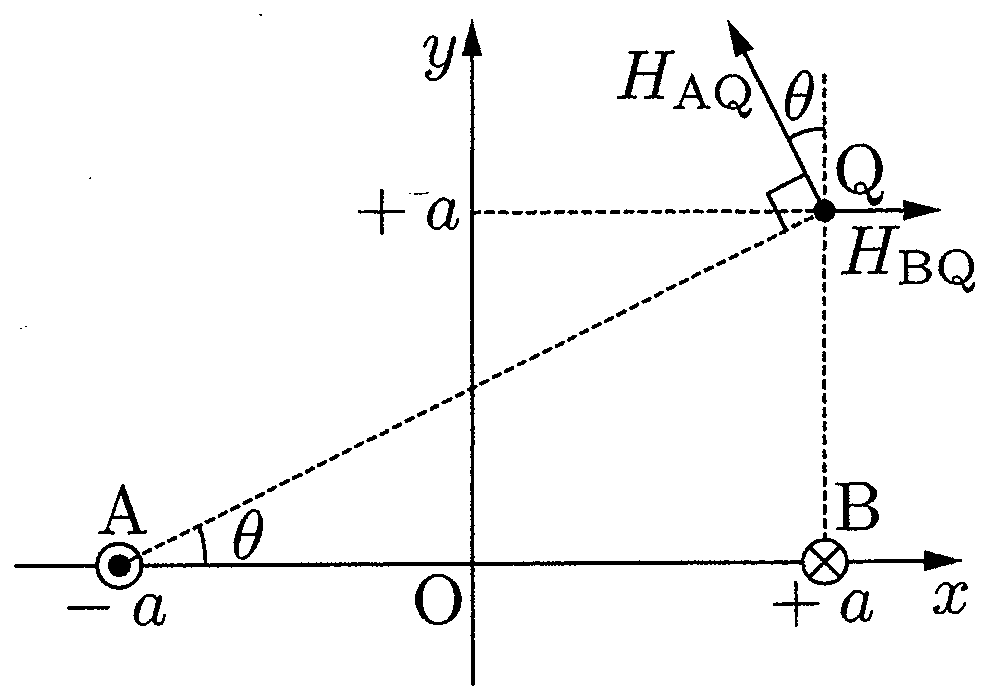
\includegraphics[keepaspectratio,width=52mm]{fig/n28_a83_zu.png}\end{center}
       合成磁場が$y$軸に平行になるためには，この二つの磁場の$x$成分が互いに打ち消し合えばよいので，$\angle\mathrm{QAB}=\theta$として，
       \[H_{\mathrm{AQ}}\sin\theta=H_{\mathrm{BQ}}\]
       であればよい．$\sin\theta=\dfrac{1}{\sqrt{5}}$を利用して上の関係式を解くと，
       \[\frac{I_1}{I_2}=5\Ans\]
\end{komon}

\MonN{84}{ソレノイドコイル}\par\nopagebreak
\begin{sisin}
ソレノイドコイル内の磁場$H=n_0I$の$n_0$は単位長さあたりの巻き数である．全巻き数と勘違いしやすいので注意すること．
\end{sisin}
\KaiHead
このコイルの単位長さあたりの巻き数$n_0$は，
\[n_0=\frac{3000}{0.2}=1.5\times 10^4\U{/m}\]
であるから，このコイルに$I\U{A}$の電流を流した場合には
\[H=n_0I=1.5\times 10^4\cdot I\U{A/m}\]
の磁場が南北に平行に作られる．地磁気によりコイル内には南北に平行にもともと$24\U{A/m}$の磁場があるのだから，これを打ち消すためには$24=1.5\times 10^4\cdot I$を満たすように電流を流せばよい．よって，
\[I=\frac{24}{1.5\times 10^4}=1.6\times 10^{-3}\U{A}\Ans\]

\MonN{85}{直線電流の作る磁場}\par\nopagebreak
\begin{sisin}
$m\U{Wb}$の磁極は$\overrightarrow{H}\U{A/m}$の磁場から$\overrightarrow{F}=m\overrightarrow{H}$で表される力を受ける．N極は正磁極であり$m>0$，またS極は負磁極であり$m<0$であるから，N極は磁場の向きに力を受け，S極は磁場と逆向きに力を受ける．その結果，磁針のN極は磁場の向きを差し示すことになる（28.1）．よって本問では，原点における合成磁場の向きを求めればよいわけである．
\end{sisin}
\KaiHead
まず，導線$\mathrm{B}$に$-y$の向きに電流$I_0\U{A}$を流すことにより原点に作られる磁場は，
\[H_{\mathrm{B}}=\frac{I_0}{2\pi\cdot\sqrt{3}a}\U{A/m}\quad(+x\text{の向き})\]
である．よって，最初，磁針は$+x$の向きを向いていることになる．この状態から導線$\mathrm{A}$に$-x$の向きに流す電流を増加させ，その強さが$I_{\mathrm{A}}\U{A}$になったときを考えると，この電流$I_{\mathrm{A}}\U{A}$が原点に作る磁場は，
\[H_{\mathrm{A}}=\frac{I_{\mathrm{A}}}{2\pi a}\U{A/m}\quad(+y\text{の向き})\]
原点の合成磁場は，この二つをベクトル合成すればよいので，合成磁場の$+x$の向きから$+y$の向きへの振れ角を$\theta$とすると，
\[\tan\theta=\frac{H_{\mathrm{A}}}{H_{\mathrm{B}}}=\sqrt{3}\frac{I_{\mathrm{A}}}{I_0}\]
である．
\begin{center}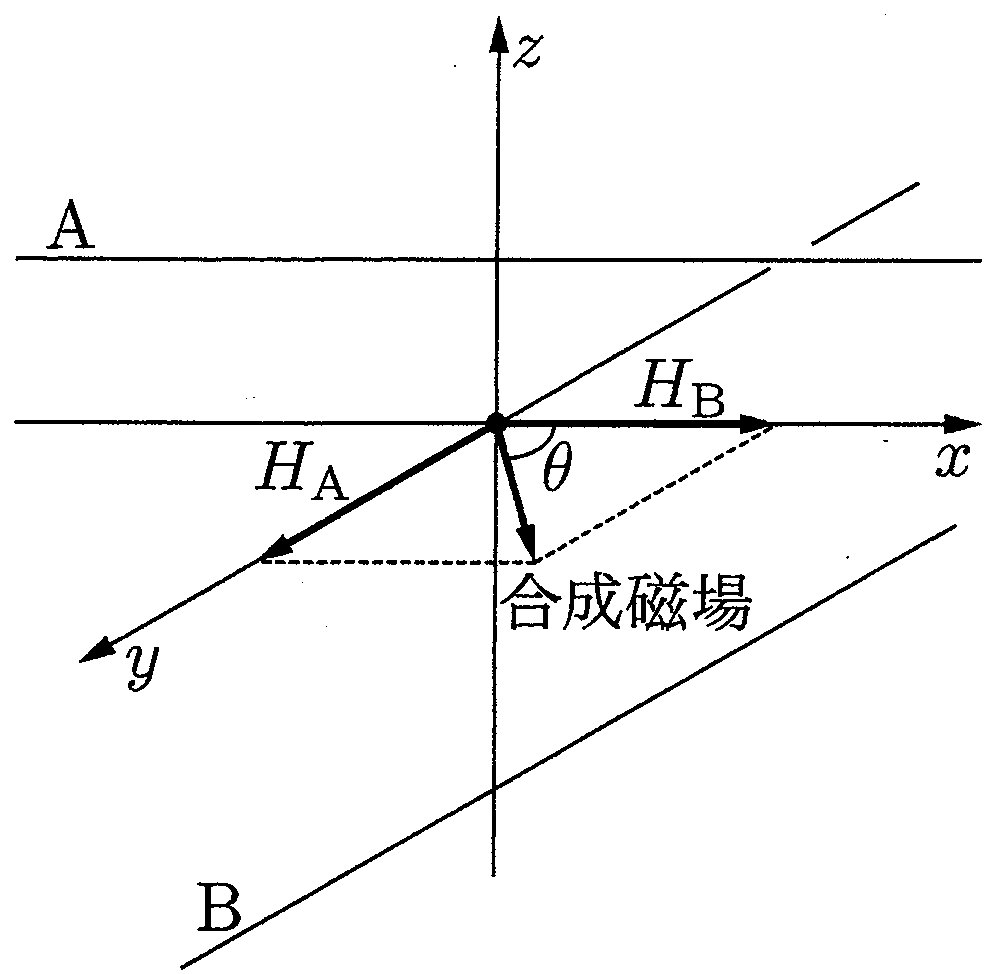
\includegraphics[keepaspectratio,width=50mm]{fig/n28_a85_zu.png}\end{center}
今，$I_{\mathrm{A}}$を$0\U{A}$から$I_0\U{A}$まで増加させると，$\tan\theta$は$0\leqq\tan\theta\leqq\sqrt{3}$の範囲で増加していくので，振れ角$\theta$は$0^\circ\leqq\theta\leqq 60^\circ$の範囲で増加していく．よって，磁針のN極と$x$軸の正の向きがなす角は
\[0^\circ\ \text{から}\ 60^\circ\ \text{へと変化していく}\Ans\]

\MonN[\Sitei]{86}{電磁力}\par\nopagebreak
\begin{sisin}
物体には，場の力である重力，電磁力，および接触力である垂直抗力の三つが作用しており，これらに対して力のつり合いの式を立てればよいが，電磁力の作用する向きに注意．電磁力は電流および磁場の両方に対して垂直な方向に作用する．力の作用の向きをはっきりさせるため，横から見た図を描くとよいだろう（28.4）．
\end{sisin}
\KaiHead
\begin{komon}
\ko{1} 導体棒には重力，電磁力，垂直抗力の三つが作用して力がつり合う．ここで，重力および垂直抗力の作用する向きは次図のようになっている．
       \begin{center}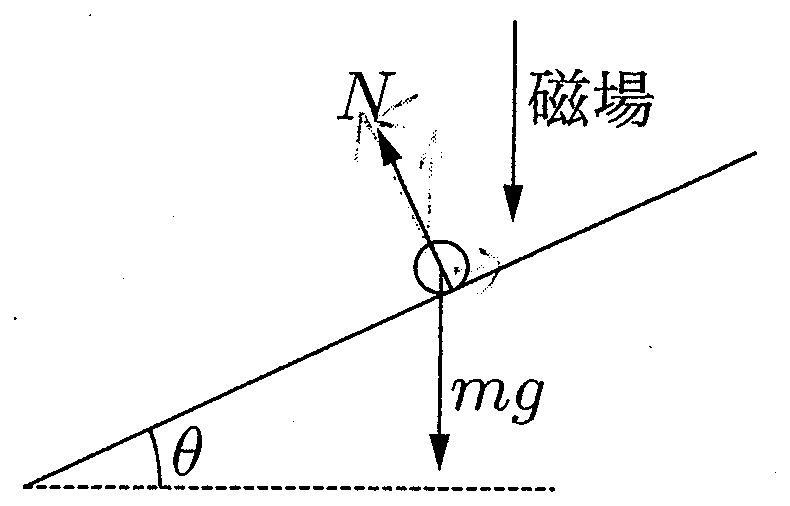
\includegraphics[keepaspectratio,width=40mm]{fig/n28_a86_zu1.png}\end{center}
       $\mathrm{PQ}$に電流を流すと，いずれの向きに流した場合であっても磁場は$\mathrm{PQ}$に水平方向の力を及ぼすことになるが，$\mathrm{PQ}$を静止させるためには，磁場が水平右向きの力を及ぼさなければならない．フレミングの左手の法則より，そのためには$\mathrm{PQ}$に対して，
       \[\mathrm{P}\to\mathrm{Q}\ \text{向き}\Ans\]
       の電流を流す必要がある．
\ko{2} 導線$\mathrm{A}$，$\mathrm{B}$が導体棒$\mathrm{PQ}$に及ぼす垂直抗力（の合力）の大きさを$N\U{N}$とする．$\mathrm{Q}$側から見た力の作用図は次図のようになる．
       \begin{center}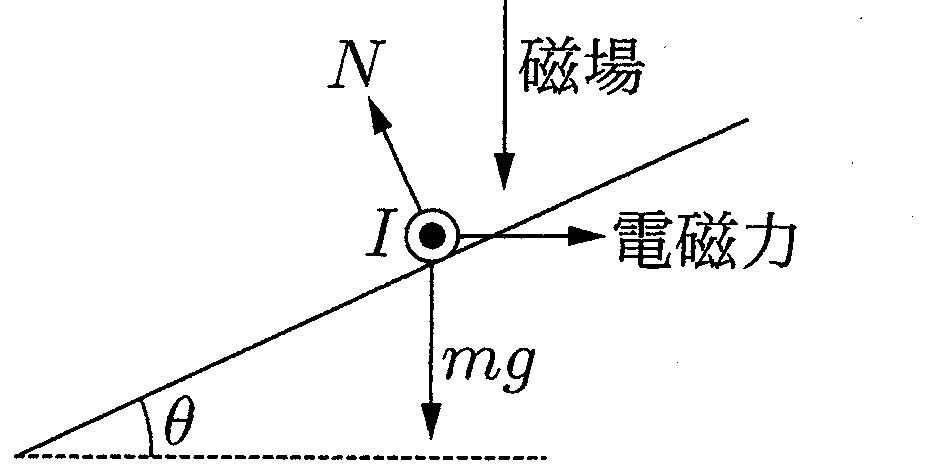
\includegraphics[keepaspectratio,width=46mm]{fig/n28_a86_zu2.png}\end{center}
       磁束密度の大きさは$B=\mu_0H\U{Wb/m^2}$であるから，導体棒$\mathrm{PQ}$に作用する電磁力の大きさは，$IBd=\mu_0IHd\U{N}$である．三つの力について，斜面方向の力のつり合いの式を立てると，
       \[mg\sin\theta=\mu_0IHd\cos\theta\]
       より，
       \[I=\frac{mg\tan\theta}{\mu_0Hd}\U{A}\Ans\]
\end{komon}

\MonN{87}{平行導線間の力}\par\nopagebreak
\begin{sisin}
$\mathrm{O}$点の磁場の強さを求めるのは単なる磁場の合成の問題なので特に問題はなかろう．(2)については，\MARU{1}まず$\mathrm{A}$，$\mathrm{B}$，$\mathrm{D}$の三つの導線が$\mathrm{C}$点に作る磁場を求めたのち，$\mathrm{C}$点の電流がこの合成磁場から受ける力を求める，という方法と，\MARU{2}二つの導線が及ぼし合う力の関係式$f=\mu_0\dfrac{I_1I_2}{2\pi r}l\U{N}$を利用して$\mathrm{A}$，$\mathrm{B}$，$\mathrm{D}$の三つの導線が$\mathrm{C}$の導線に対して及ぼす力を求め，この力の合力を取る，というやり方の2通りが考えられる．どちらでももちろん同じ答えが求められる．ここでは前者の考え方で解答を示すが，後者の考え方でも解いてみて欲しい．
\end{sisin}
\KaiHead
\begin{komon}
\ko{1} $\overline{\mathrm{OA}}=\overline{\mathrm{OB}}=\overline{\mathrm{OC}}=\overline{\mathrm{OD}}=\dfrac{a}{\sqrt{2}}\U{m}$であるから，各導線が$\mathrm{O}$点に作る磁場の強さはいずれも
       \[H=\frac{I}{2\pi(a/\sqrt{2})}\U{A/m}\]
       である．右ねじの法則を利用すると，各導線が作る磁場の向きはそれぞれ次図の通りである．
       \begin{center}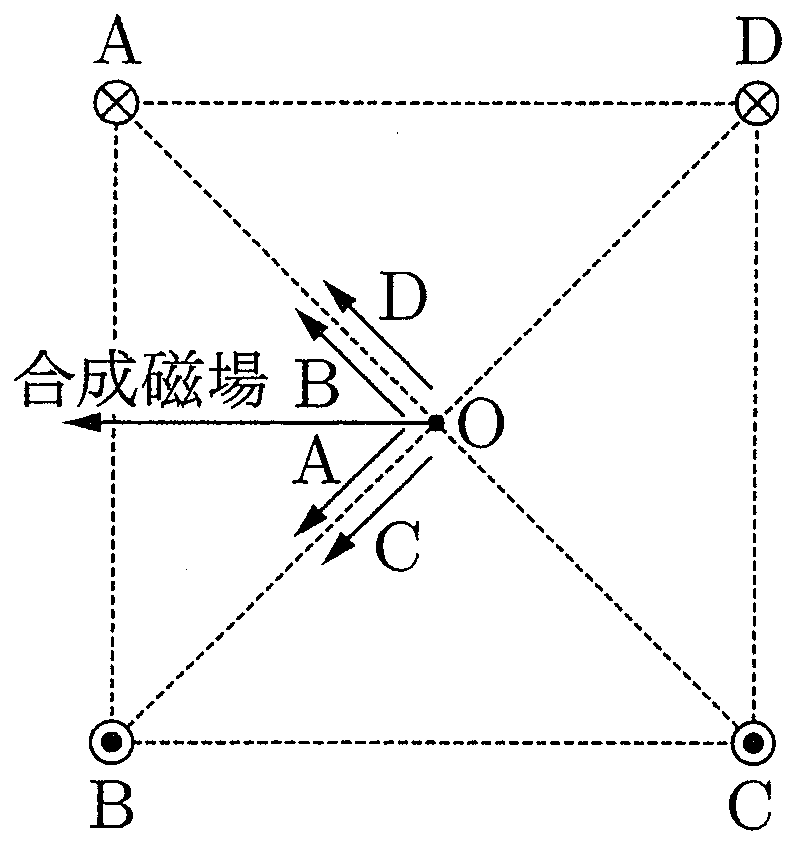
\includegraphics[keepaspectratio,width=44mm]{fig/n28_a87_zu1.png}\end{center}
       よって，この四つの磁場を合成すると$\overrightarrow{\mathrm{DA}}$の向きになり，その強さは，
       \[H_{\mathrm{O}}=4\times\frac{H}{\sqrt{2}}=\frac{2I}{\pi a}\U{A/m}\Ans\]
\ko{2} $\overline{\mathrm{AC}}=\sqrt{2}a\U{m}$，$\overline{\mathrm{BC}}=\overline{\mathrm{DC}}=a\U{m}$であることに注意して，$\mathrm{A}$，$\mathrm{B}$，$\mathrm{D}$の導線が$\mathrm{C}$の導線の位置に対して作る磁場$H_{\mathrm{A}}^\prime$，$H_{\mathrm{B}}^\prime$，$H_{\mathrm{D}}^\prime\U{A/m}$を求めると，強さはそれぞれ
       % 原本は H'_B, H'_D が立体の H になっていた．
       \[H_{\mathrm{A}}^\prime=\frac{I}{2\pi\sqrt{2}a},\quad H_{\mathrm{B}}^\prime=H_{\mathrm{D}}^\prime=\frac{I}{2\pi a}\]
       であり，向きは次図の通りである．
       \begin{center}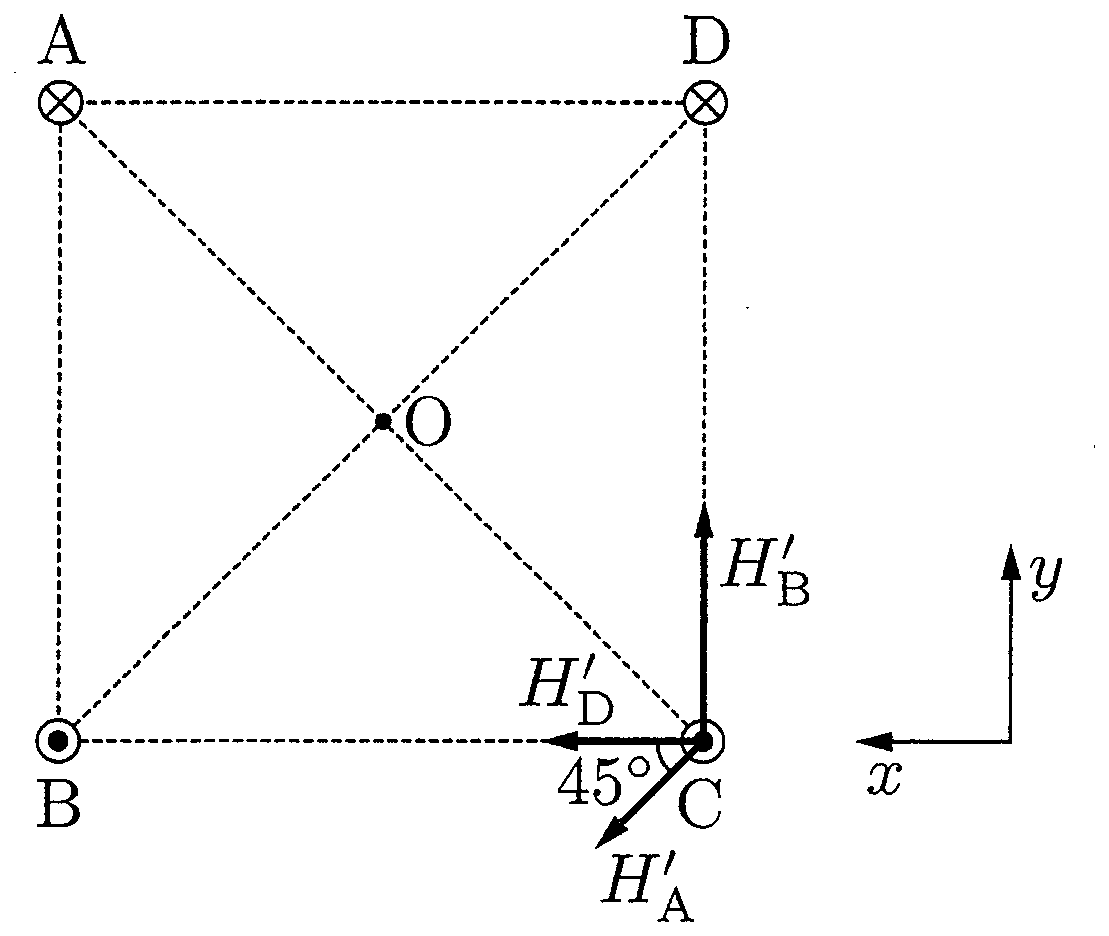
\includegraphics[keepaspectratio,width=48mm]{fig/n28_a87_zu2.png}\end{center}
       前図のように$x$，$y$各軸方向を取り，成分計算によってこの三つの磁場を合成すると，合成磁場$\overrightarrow{H}$は
       \[\begin{aligned}
         \overrightarrow{H}&=(H_{\mathrm{D}}^\prime+H_{\mathrm{A}}^\prime\cos 45^\circ,\ H_{\mathrm{B}}^\prime-H_{\mathrm{A}}^\prime\sin 45^\circ)\\
         &=\Bigl(\frac{3I}{4\pi a},\ \frac{I}{4\pi a}\Bigr)\U{A/m}
       \end{aligned}\]
       である．導線$\mathrm{C}$はこの合成磁場から次図のように力を受ける．
       \begin{center}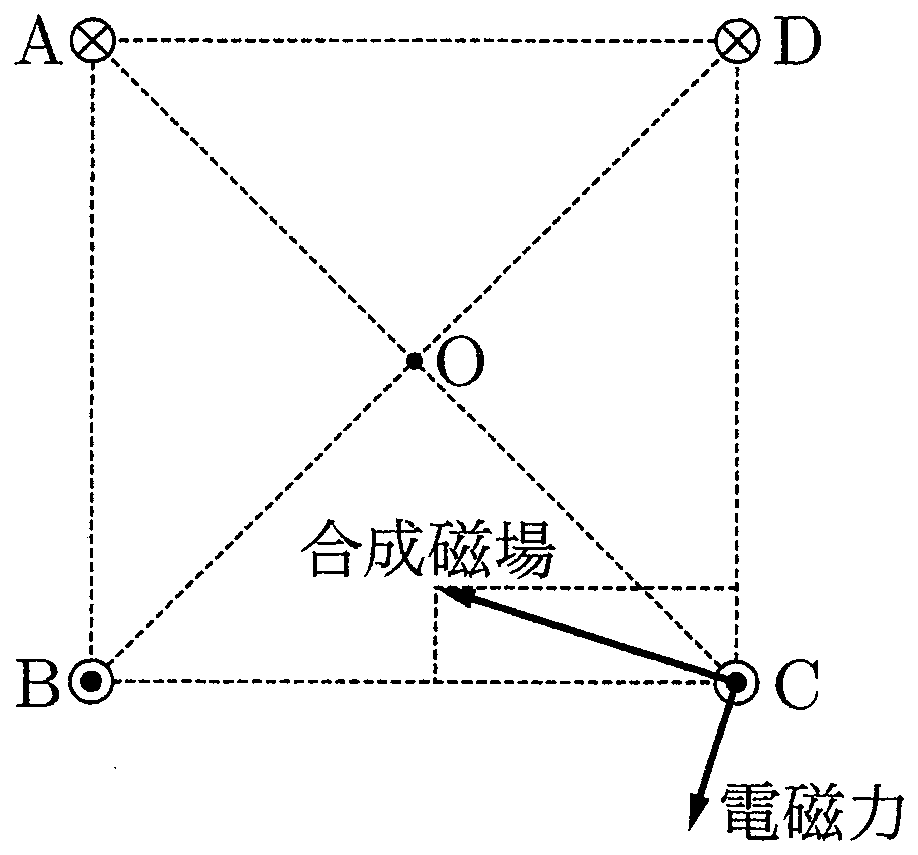
\includegraphics[keepaspectratio,width=46mm]{fig/n28_a87_zu3.png}\end{center}
       よって，導線$\mathrm{C}$の$1\U{m}$あたりに作用する電磁力の大きさは，
       \[f_{\mathrm{C}}=(\mu_0|\overrightarrow{H}|)\cdot I\cdot 1=\frac{\sqrt{10}\mu_0I^2}{4\pi a}\U{N}\Ans\]
\end{komon}

\Rank{C問題}
\MonN{88}{部分円電流の作る磁場}\par\nopagebreak
\begin{sisin}
任意の形状の電流が作る磁場は，原理的にはビオ・サバールの法則を利用して求めることができるが，これを計算するには高度な数学が要求されるため，高校範囲ではこれを利用して求めることはほぼ不可能である．そこで本問のような，いくつかの組み合わせで作られているような導線については，磁場についての重ね合わせの原理を利用して考える．

問題文中にもあるが，一般に，ある平面上を流れる電流が，その平面内の点に作る磁場の向きは，導線の形によらずその平面に対して垂直になる（28.3）．このことと重ね合わせの原理を利用すれば，$\mathrm{O}$点での磁場の強さが求められるはずである．
\end{sisin}
\KaiHead
\begin{komon}
\ko{1} 次図のように，この電流と点$\mathrm{O}$に関して$120^\circ$，$240^\circ$だけ回転させた電流とを組み合わせると一つの円形電流のみとなる（半径部分の電流は互いに打ち消し合う）．
       \begin{center}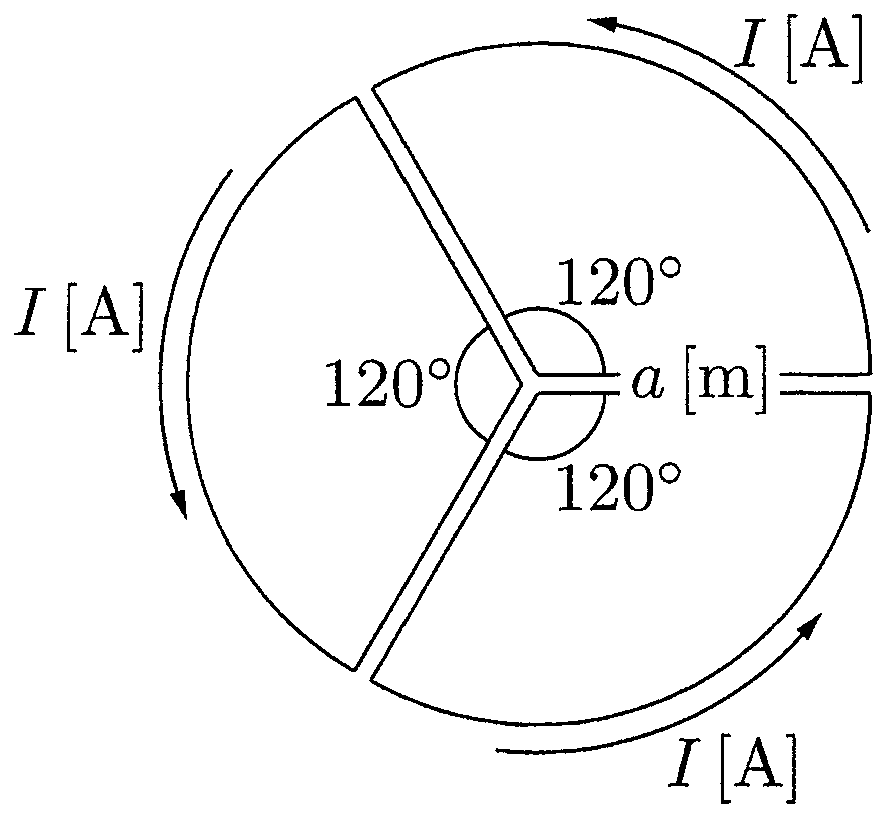
\includegraphics[keepaspectratio,width=44mm]{fig/n28_a88_zu1.png}\end{center}
       各$120^\circ$部分が点$\mathrm{O}$に作る磁場は同じ大きさであるから，一つあたり点$\mathrm{O}$に$H\U{A/m}$の磁場を作っているとすると，$3\times H=\dfrac{I}{2a}$が成立する．よってこれを解いて，
       \[H=\frac{I}{6a}\U{A/m}\Ans\]
       （向きは紙面に対して裏→表向きである）
\ko{2} 次図のようにこの電流（実線）と点$\mathrm{O}$に関して$180^\circ$だけ回転させた電流（破線）とを組み合わせると，互いに逆向きに流れる2本の直線電流と円形電流を組み合わせたものとなる．
       \begin{center}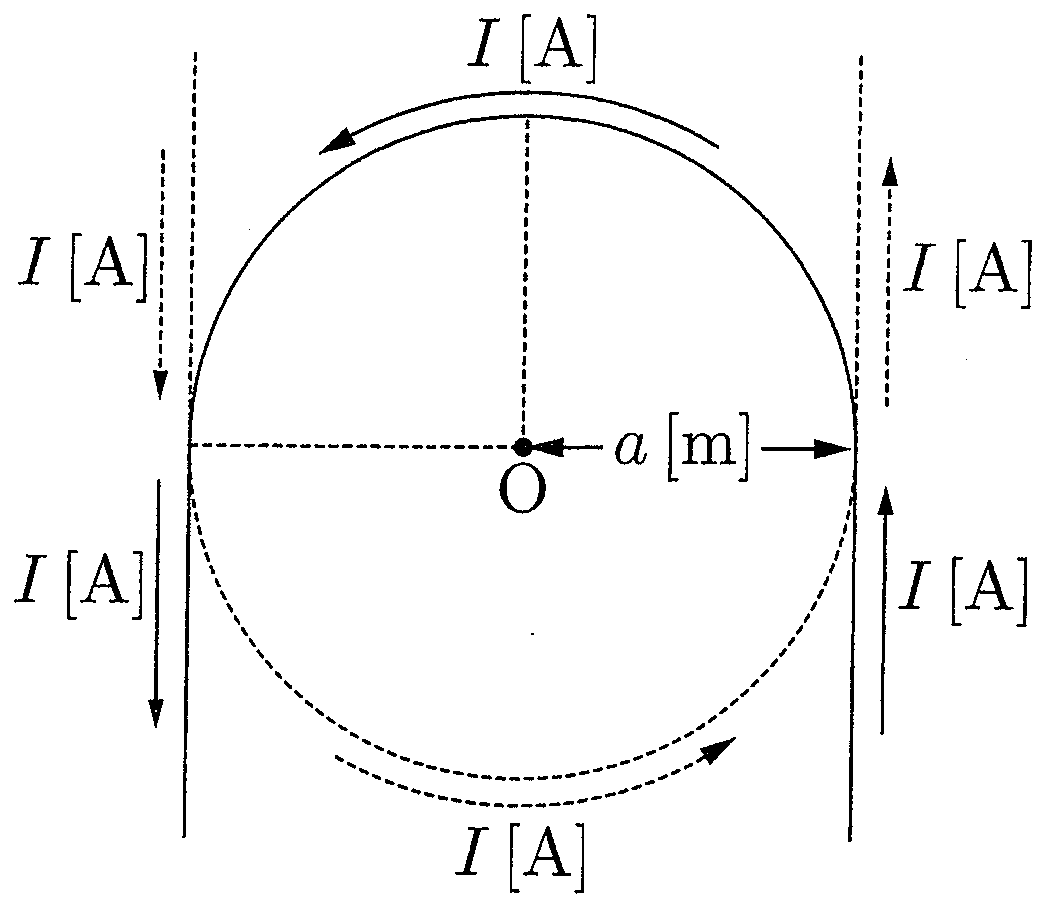
\includegraphics[keepaspectratio,width=48mm]{fig/n28_a88_zu2.png}\end{center}
       実線と破線の各電流が点$\mathrm{O}$に作る磁場は同じ大きさであるから，一つあたり点$\mathrm{O}$に$H\U{A/m}$の磁場を作っているとすると，
       \[2\times H=\frac{I}{2a}+\frac{I}{2\pi a}+\frac{I}{2\pi a}\]
       が成立する（円形電流および直線電流2本が作る磁場はいずれも紙面に対して裏→表の向きである）．よってこれを解いて，
       \[H=\frac{(2+\pi)I}{4\pi a}\U{A/m}\Ans\]
       （向きは紙面に対して裏→表向きである）
\end{komon}

\MonN{89}{長方形コイルが受ける力}\par\nopagebreak
\begin{sisin}
辺$\mathrm{AD}$，$\mathrm{BC}$が受ける力を考える際，導線$\mathrm{PQ}$に流れる電流が辺上に作る磁場は辺上の各点ごとに異なるため，辺$\mathrm{AD}$，$\mathrm{BC}$が受ける力を求めるためには，まず辺を微小区間に区切り，各微小区間が受ける力を求めてこれを足し合わせるという面倒な計算を行わなければならない．しかし，辺$\mathrm{AD}$，$\mathrm{BC}$に流れる電流は互いに逆向きであるため，各辺にかかる力を同時に考えると打ち消し合ってしまう．このことをうまく説明して(2)を求めよう．
\end{sisin}
\KaiHead
\begin{komon}
\ko{1} 右ねじの法則より，導線$\mathrm{PQ}$が辺$\mathrm{AB}$，$\mathrm{CD}$の位置に作る磁場はいずれも紙面に垂直で，表→裏の向きである．またその強さは，
       \[H_{\mathrm{AB}}=\frac{I_1}{2\pi d},\quad H_{\mathrm{CD}}=\frac{I_1}{2\pi(d+b)}\]
       である．導線$\mathrm{PQ}$はこの磁場により辺$\mathrm{AB}$，$\mathrm{CD}$の導線に力を及ぼす．この磁場から辺$\mathrm{AB}$，$\mathrm{CD}$の導線が受ける力の大きさは，
       \[\left\{\begin{aligned}
         f_{\mathrm{AB}}&=(\mu_0H_{\mathrm{AB}})I_2a=\frac{\mu_0I_1I_2a}{2\pi d}\U{N}\\
         f_{\mathrm{CD}}&=(\mu_0H_{\mathrm{CD}})I_2a=\tfrac{\mu_0I_1I_2a}{2\pi(d+b)}\U{N}
       \end{aligned}\right.\Ans\]
       であり，電流の向きに注意するとフレミングの左手の法則より，それぞれ左向き，右向きに作用している．
       \begin{chuu}
       $f_{\mathrm{AB}}$，$f_{\mathrm{CD}}$の向きは，二つの電流が同じ向きか逆向きかでも簡単に把握できる（同じ向きは引力，逆向きは斥力）．
       \end{chuu}
\ko{2} 導線$\mathrm{PQ}$がコイル$\mathrm{ABCD}$に及ぼす力とは，$\mathrm{PQ}$がコイルの各辺$\mathrm{AB}$，$\mathrm{BC}$，$\mathrm{CD}$，$\mathrm{DA}$に及ぼす力の合力のことである．辺$\mathrm{BC}$，$\mathrm{DA}$にかかる力を以下の手順で考える．

       $\mathrm{BC}$，$\mathrm{DA}$上の，$\mathrm{PQ}$から$x\U{m}$（$d\leqq x\leqq d+b$）だけ離れた点に着目し，$x\sim x+dx$の長さ$dx\U{m}$の微小部分について考える．導線$\mathrm{PQ}$に流れる電流はこの部分に紙面に垂直で，表→裏の向きの磁場を作り，その強さは$H(x)=\dfrac{I_1}{2\pi x}\U{A/m}$で与えられる．この磁場により，$\mathrm{BC}$，$\mathrm{DA}$上の長さ$dx$の微小部分は次図のような向きにそれぞれ大きさ$f=\mu_0H(x)\cdot I_2\cdot dx\U{N}$の電磁力を受ける．
       \begin{center}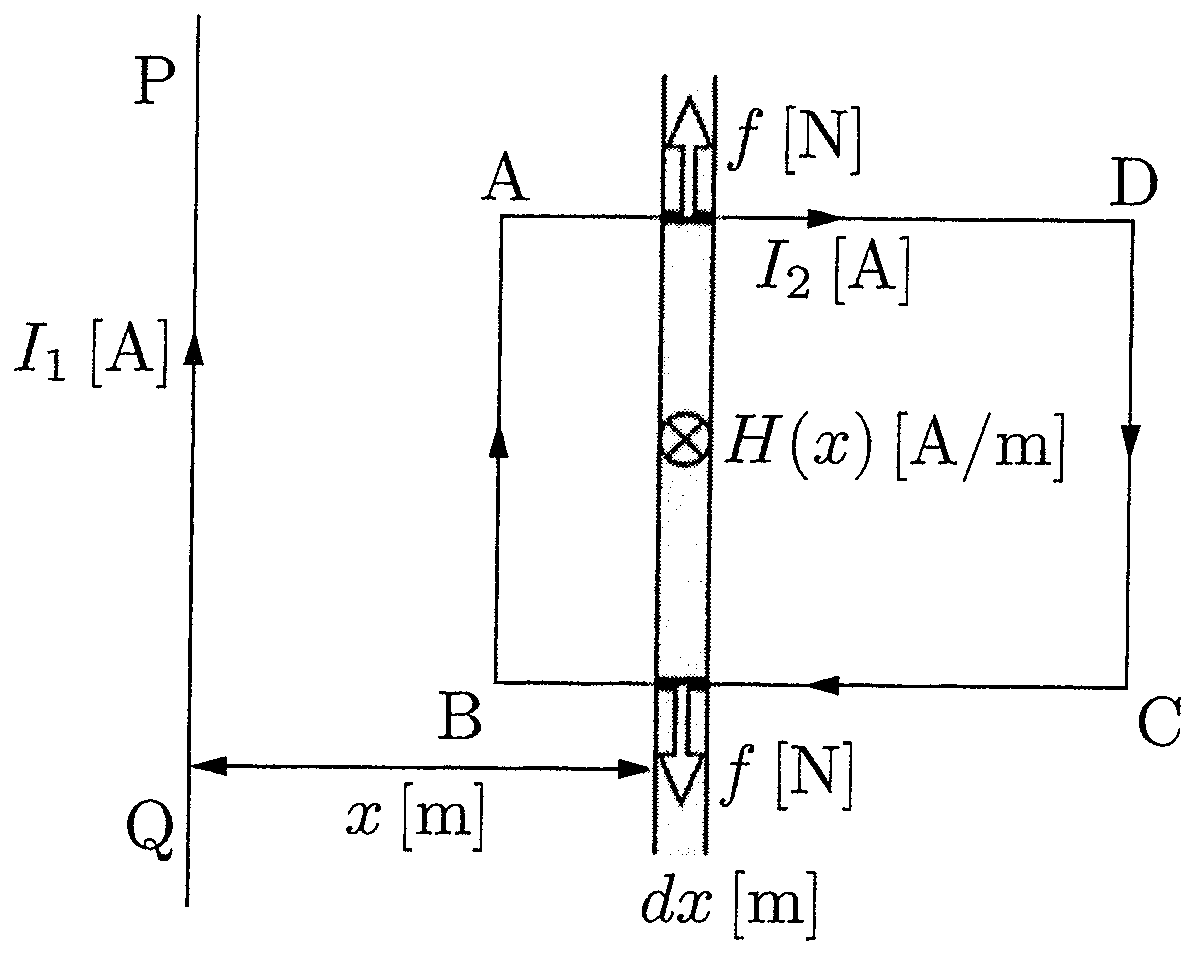
\includegraphics[keepaspectratio,width=52mm]{fig/n28_a89_zu.png}\end{center}
       ところが前図から分かるように，この二つの力は等大逆向きであるから互いに打ち消し合う．すなわち，辺$\mathrm{BC}$，$\mathrm{DA}$にかかる電磁力は，導線$\mathrm{PQ}$から同一距離にある点同士が打ち消し合い，結果として辺$\mathrm{BC}$，$\mathrm{DA}$にかかる電磁力の合力は$0$となる．

       以上より，コイルの各辺に及ぼす力の合力は辺$\mathrm{AB}$，$\mathrm{CD}$の二つにかかる力の合力$f_{\mathrm{AB}}-f_{\mathrm{CD}}$となるので，(1)の結果を利用して（$f_{\mathrm{AB}}>f_{\mathrm{CD}}$であることに注意して），
       \[\left\{\begin{aligned}
         &\text{向き：}\ \overrightarrow{\mathrm{DA}}\ (=\overrightarrow{\mathrm{CB}})\ \text{の向き}\\
         &\text{大きさ：}\ \frac{\mu_0I_1I_2ab}{2\pi d(d+b)}\U{N}
       \end{aligned}\right.\Ans\]
\end{komon}
\begin{bsHosoku}{参考}
導線$\mathrm{PQ}$が辺$\mathrm{BC}$に及ぼす力は，上で求めた微小部分$dx$に働く力を足し合わせることで求められる．微小量の足し合わせは積分であるから，
\[\begin{aligned}
  f_{\mathrm{BC}}&=\int_d^{d+b}\frac{\mu_0I_1I_2}{2\pi x}dx=\frac{\mu_0I_1I_2}{2\pi}\bigl[\log|x|\bigr]_d^{d+b}\\
  &=\frac{\mu_0I_1I_2}{2\pi}\log\Bigl(1+\frac{b}{d}\Bigr)\U{N}
\end{aligned}\]
として求めることができる．
\end{bsHosoku}

\end{multicols}
